\chapter{Heuristic Decision Making in a Social Economic Model of Fossil Resource Usage}
\label{chapter:heuristics}
This chapter is based on unpublished work. However, a simplified version of the economic model is part of \citep[P5]{Kolb2019b}.
\section{Introduction}

In the IPCCs current business as usual scenarios, the CO$_{2}$ emissions budget that limits global warming to below 1.5$^{\circ}$C with a likelihood of 0.5 will be exceeded by approximately 2030. This means that in order to limit global warming below 1.5$^{\circ}$C, the global economy needs a rapid shift away from fossil fuel based technologies. Currently, the two main measures that are expected to incentivize the necessary changes are taxation and cap and trade schemes for CO$_{2}$ emissions. I suspect that these measures are favoured by many because they are expected to be efficient. This is most likely because their effects are thought to be adequately understood as they can be estimated well with the current integrated assessment models that are used to generate the economic projections for the IPCCs reports. However, there are some issues with these policy measures. First, the expected effects of these policy measures are estimated in an idealized model world whereas their real effects come from their real implementation that might include a number of exceptions, loopholes and unintended consequences. And second, with few exceptions, the political process to implement these measures is sluggish and the outcomes are all but certain.

Therefore, I argue that in addition to top down policy measures, bottom up initiatives are essential to successfully mitigate global warming. 
There are a number of such bottom up initiatives such as Fridays for Future or Extinction Rebellion that are currently gaining more and more traction. These initiatives use means of collective and direct action make their claims and to influence public discourse. The analysis of similar movements shows that their dynamics are essentially driven by opinion formation and individual decision processes amongst heterogeneous individuals \citep{Graeber2009, Engler2016}. Consequently, as discussed in section \ref{sec:intro_complex_systems}, the models that are currently used for climate change mitigation scenarios are unable to picture them due to their reliance on a representative agent approach.

With this motivation I develop a conceptual economic model of fossil resource use and technological change that is able to explicitly depict individual decision making of heterogeneous agents, as well as social learning and opinion formation in order to better understand the possible effects of social movements in mitigating global warming.

This model combines individual decision making via a simple fast and frugal decision heuristic and interactions between individuals via a social learning process with feedbacks on an aggregated supply and demand level in a two sector investment economy.

In the reminder of this chapter, I will outline and explain this model in section \ref{sec:heuristics_model}, simplify it analytically as far as possible and explore some of its limiting cases in sections \ref{sec:algebraic_constraints} and \ref{sec:limiting_cases} and fit its parameters to past economic data in section \ref{sec:parameter_values}. Subsequently, I analyze the models default dynamics in section \ref{sec:default_scenario} and showcase the possibility to analyze a stylized social movement with this model in section \ref{sec:campaign} before concluding.

\section{Model Development}  
\label{sec:heuristics_model}
Previous studies by \cite{Ans2013} suggest that feedback through supply-demand price mechanisms will have only limited impact on fossil fuel companies. This is due to the fact that only approximately 15 \% of investors invest subject to socially responsible guidelines \citep{SIF2014Report} and that divested holdings are, especially in liquid markets, very likely to quickly find their way to less responsible investors. \\
Also, as long as the physical capital relying on fossil fuels already exists, economic reasoning follows that it will be used as long as variable costs are covered.
Therefore, a general economic shift from dirty to clean technology needs changes in investment in physical capital or a political imperative mandated by a (qualified) majority. Therefore, I consider a model focussing on savings and investment decisions appropriate to investigate the possible dynamics of an economic transition towards fossil resource independent technologies.\\
In the following I propose a preliminary scheme of such a model.
\begin{figure}[t]
	\centering
	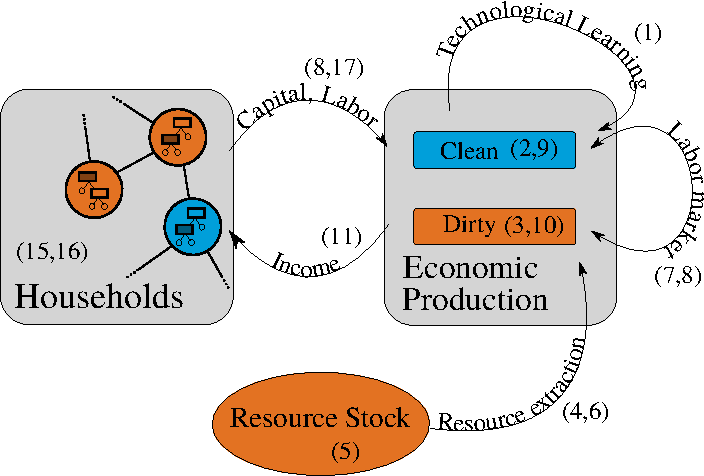
\includegraphics[width =.8 \textwidth]{figures/model_scheme_1.pdf}
        \caption[Schematic sketch of a two sector investment model with heterogeneous households that are bounded rational decision makers]{Schematic sketch of the model consisting of two production sectors (a \emph{clean} and a \emph{dirty} one) and heterogeneous households that are heuristic decision makers that interact on a complex adaptive acquaintance network. Households supply labor and capital to the production sectors. The production sectors each have their separate capital market but are linked via a shared labor market. The \emph{dirt} sector depends on the input of an exhaustible fossil resource, the \emph{clean} sector depends on a developing technology that is endogenously modelled via learning by doing. Boxes and bubbles signify modelled entities, arrows signify interactions. Numbers ($x$) next to entities and interactions give the decimal place of equations in the model description section \ref{sec:model_description} that describe the respective processes.}
	\label{fig:model}
\end{figure}

\subsection{Economic Production}
\label{sec:model_description}

As illustrated in \cref{fig:model}, the model consists of two sectors for production and a set of heterogeneous households that interact via an adaptive complex social network. The production sectors employ different technology. I call them the \textit{clean} and the \textit{dirty} sector for illustrative clarity. The heterogeneous households in the model provide capital $K$ and labor $L$ to both sectors.
In addition, the production technology in the dirty sector depends on the input of an exhaustible (fossil) energy-resource $R$ that is used up in the process. I assume that the technology in the dirty sector is fully developed and adequately described in terms of the total factor productivity. 
Price elasticities\footnote{The price elasticity of demand ($PED$) for a good describes the change in demand $Q$ for that good when the price of that good $P$ (and nothing else) changes. Formally, it is defined as $PED = \partial Q / \partial P \times P/Q$. Informally this means that if the price elasticity of a good is low, it will be bought in similar quantities regardless of rising prices.} of demand for fossil fuel are evidently low in real economies \citep{IMF2011, Hosslinger2017, Labandeira2017}, even with the choice between alternative technologies factored in. I approximate this by setting the marginal rate of substitution\footnote{The marginal rate of substitution $MRS_{12}$ of two goods $G_1$ and $G_2$ describes the extent to which good $G_1$ can be replaced by good $G_2$ in a given economic process. More precisely, in this case it would be called the marginal rate of \emph{technical} substitution as it refers to the substitution of two goods in a production process (as opposed to the substitution of goods in consumption). Technically, it is defined as 
\begin{equation}
  MRS_{12} = \frac{\partial Y(G_1,G_2)}{\partial G_1} / \frac{\partial Y(G_1, G_2)}{\partial G_2} \nonumber
\end{equation}
where $Y(G_1, G_2)$ is the economic production function that links the input of goods $G_1$ and $G_2$ to economic output $Y$. In effect, this means that when the marginal rate of technical substitution between two goods is zero, they cannot be replaced by one another in a production e.g., when one of the goods is missing, production halts regardless of the quantities of the other good that are available.} between the fossil resource and the pair of capital and labor to zero in the dirty sector. This is also in line with contemporary critique of the neoclassical growth models \citep{Daly1997,georgescu1975energy,georgescu1979comments, Ayres2007, Ayres2013} that highlights the generally assumed substitutability of natural resources in production as being physically implausible and lacking empirical evidence.

I acknowledge the common argument for substitutability between capital, labor and energy resources due to a shift in the output of economic production from manufacturing to services and would argue that this model pictures this in a shift of economic production from the dirty sector to the clean one which is described in the following.

The clean sector represents a circular economy in which the output of final goods depends on the machinery, knowledge and effort used in its production and is not limited by entropy laws or resource scarcity on the timescale under consideration. The technology $C$ used in the clean sector is assumed to be still in development and is therefore explicitly modeled.
Following \cite{argote1990learning}, I model technological process as learning by doing according to Wright's law \citep{wright1936factors, Nagy2013} with a one-factor learning curve. I assume that $C$ is proportional to cumulative production but also depreciates with a constant rate $\chi$. 
\begin{equation}
	\dot{C} = Y_c - \chi C.
	\label{eq:learning_by_doing}
\end{equation}
Depreciation can be regarded as a human capital effect that leads to knowledge depreciation over time \citep{Kahouli-Brahmi2008}. This is also in line with the empirically observed decrease in learning rates for maturing technologies \citep{argote1990learning}
In the clean sector, capital $K$, labor $L$ and technology/knowledge $C$ are assumed to be mutual substitutes. To satisfy these requirements, I use the following production functions:
\begin{align}
	Y_c &= b_c C^{\gamma} L_c^{\alpha_c}K_c^{\beta_c}, \label{eq:clean_production} \\
	Y_d &= \mathrm{ min}\left( b_d L_d^{\alpha_d}K_d^{\beta_d}, e R \right), \label{eq:dirty_production}
\end{align}
Subscripts $c$ and $d$ denote the clean and dirty sector respectively, $Y_c$ and $Y_d$ are their economic outputs and $L_c$ and $L_d$ are labor shares in each sector. $\alpha$ and $\beta$ are elasticities of the respective input factors and $b_c$ and $b_d$ are the total factor productivity and $K_c$ and $K_d$ are the capital stocks for the respective sector.
% Measuring unit production cost in the number of working hours as in the original study by Wright \cite{wright1936factors}, $\gamma$ is equivalent the elasticity of learning by doing in the clean sector as outlined in \cite{Kahouli-Brahmi2008}.
% This is probably too much info and confusing for a physics audience.

The structure of eq. \ref{eq:dirty_production} implies that if $b_d L_d^{\alpha_d}K_d^{\beta_d} \ne e R$, either capital and labor or fossil resource would be available in excess but unused and idle, which would be inefficient. I assume efficient an usage of resources in the dirty sector, such that
\begin{equation}
    b_d L_d^{\alpha_d}K_d^{\beta_d} = e R
    \label{eq:efficient_dirty_resources}
\end{equation}
where $1/e$ is the resource intensity of the sector. The usage of the fossil resource $R$ depletes a geological resource stock $G$ with the initial stock $G(t=0) = G_0$:
\begin{equation}
    \dot{G} = -R. 
    \label{eq:resource_depletion}
\end{equation} 
In line with the assumptions common in the literature \citep{Dasgupta1974, Perman2003}, the total cost $c_R$ for the usage of the fossil resource depends on the resource use $R$ and the remaining fossil resource stock $G$ such that total resource costs increase with resource use ($\partial c_R / \partial R >0$) and also with continued resource depletion ($\partial c_R / \partial G < 0$). I chose the specific form to be
\begin{equation}
	c_R = b_R R^{\rho}\left( \frac{G_0}{G} \right)^{\mu}; \quad \rho \geq 1, \quad \mu > 0,
	\label{eq:resource_cost}
\end{equation}
such that at some point $\partial Y_d / \partial R < \partial c_R / \partial R$ to take into account that some part of the resource is not economic, e.g. its marginal cost exceeds its marginal productivity.
Perfect labor mobility and competition for labor between the two sectors lead to an equilibrium wage $w$ that equals the marginal return for labor:
\begin{equation}
	w = \frac{\partial Y_c}{\partial L_c} = \frac{\partial Y_d}{\partial L_d} - \frac{\partial c_R}{\partial L_d}
	\label{eq:equilibrium_wage}
\end{equation}
with the sum of the labor shares equal to the total amount of labor available:
\begin{equation}
	L_c + L_d = L.
	\label{eq:population}
\end{equation}
I assume physical capital to be specific to the technology employed such that it can only be used in the sector that it has been invested in originally, resulting in separate capital markets for the two sectors. I assume these capital markets to be fully competitive resulting in capital rents equal to marginal productivity:
\begin{align}
	r_c &= \frac{\partial Y_c}{\partial K_c} \label{eq:clean_capital_rent}\\
	r_d &= \frac{\partial Y_d}{\partial K_d} - \frac{\partial c_R}{\partial K_d} \label{eq:dirty_capital_rent}
\end{align}

\subsection{Investment Decision Making}
\label{sec:investment_decision_making}
I model households as bounded rational decision makers \citep{simon1972theories, simon1982models, gigerenzer2002bounded}.
That is, households take their investment decisions, i.e. whether to invest their savings in the clean or the dirty sector, not by forming rational expectations \citep{Evans2006, Kirman2014} but by A) using \emph{heuristic decision strategies} to make robust decisions with sparse information and with limited computational work and B) engaging in \emph{social learning} \citep{Bandura1971} to obtain successful decision strategies \citep{Traulsen2010} with reasonable effort.

% Why use Fast and Frugal heuristics for decision making?
Regarding individual decision making, there is ample evidence that real investors rather use a diverse set of heuristic strategies to make investment decisions. \cite{Gigerenzer2018} and other researchers in the field strongly suggest to consider these so called \emph{Fast and Frugal heuristic} decision models as a complementary alternative to established probabilistic and optimizing decision models. 
In general, Fast and Frugal Heuristics are described in terms of three building blocks; one for information search, one for stopping information search and one for evaluating the available information and drawing a conclusion from it.
I use a decision heuristic called \emph{Take The Best} that is observed to be frequently used in situations where individuals need to decide between one of two options that are comparable in different aspects \citep{gigerenzer1999simple, Newell2003a}. 
Take the Best has the following building blocks: 1) Search through cues in a predefined order, 2) stop as soon as one cue discriminates between the two options, 3) chose the option with the preferable value on the discriminating cue. \\
This requires a so called \textit{cue order} e.g.\ a hierarchy of validity for the pieces of information that are considered relevant for the decision. \\

% How these heuristics can be interpreted in this context.
Research on perception and decision making in psychology where the concept of Fast and Frugal heuristics was developed usually considers inferential decisions (since they have true and false outcomes and can therefore be benchmarked and evaluated statistically).\\
Nevertheless, Heuristic decision making is a reasonable tool for preferential decisions as well. Although in this context the interpretation of cue orders would be different - namely, they would rather be considered as norms or underlying preferences that apply to the context of the decision. \\
The case of savings decisions that is considered in this model poses an intermediate case between preferential and inferential decisions for a number of reasons. First, there is no immediate feedback on savings decisions, since the return on investment depends on the future development of the economic system which again depends on the savings decisions of all other households and second, I assume that households do not only consider financial but also moral grounds for their savings decisions.
Additionally, I argue that imitation of peers is not only an efficient learning strategy in many situations but also a value in its own - especially if the question is to some extend ethical. 

% Heuristics can be learned from others. This is why we model social learning.
Nevertheless, some strategies are suspected to have more profitable long term results then others as the performance of this decision heuristic depends on the order of the sequence of cues \citep{Gigerenzer2011}. Empirical evidence shows that if participants in an experiment are allowed to share information about their cue orders and respective performance, they do so and thereby greatly increase the speed of learning of cue orders that fit their decision environment compared to individual trial and error reinforcement learning \citep{garcia2009does}. Therefore, I use social learning among households to determine the particular cue order that determines their investment decision making.

% As the outcomes of social learning depend on network topology, we model topology endogenously.
As the outcomes of social learning crucially depend on the structural properties of the complex network of social ties amongst the households \citep{Barkoczi2016}, I model the adaptive formation of this social network endogenously.
A well established principle for the emergence of structured ties in social networks is homophily, i.e. the tendency that similar individuals are linked \citep{McPherson2007, Centola2007, Centola2011}. Especially the concept of value homophily \citep{McPherson2007} is in line with the interpretation of cue orders above not only as a means to the end of making profitable investment decisions but also as an expression of identity and beliefs with regards to clean technology.
The following model specification uses social learning in combination with endogenous network adaptation based on homophily to model the changes in heuristic decision strategies that households use to make investment decisions.

% How I do this technically (Individual Household earnings and investment)
I model $N$ heterogeneous households denoted with the index $i$ as owners of one unit of labor $L^{(i)} = L/N$ and capital $K_c^{(i)}$ and $K_d^{(i)}$ in the clean and dirty economic sector respectively.
Households generate an income $I^{(i)}$ from their labor and capital income which they use for consumption $F^{(i)}$ and savings $S^{(i)}$:
\begin{align}
	I^{(i)} &= w L^{(i)} + r_c K_c^{(i)} + r_d K_d^{(i)}, \label{eq:household_income} \\
	F^{(i)} &= (1-s) I^{(i)}, \label{eq:consumption} \\
	S^{(i)} &= s I^{(i)}. \label{eq:savings}
\end{align}
A binary decision parameter $o_i \in [c,d]$ denotes the sector in which the households decide to invest and $s$ denotes the savings rate at which households reinvest their income. As motivated above, I model decision making that is driven by three processes: Heuristic decision making via the Take The Best heuristic, social learning via the imitation of successful cue orders and homophily towards individuals exhibiting the same beliefs as represented by its cue order. \par

% How I do this technically (Heuristic and cue order here)
Concerning the information that households use to make their investment decisions, they are assumed to be unable to form rational expectations about the future, e.g.\ they make decisions based solely upon information about the past and present. Possible sources of information are economic indicators such as capital rents in both sectors $r_c$ and $r_d$ and their trends $\dot{r}_c$ and $\dot{r}_d$ as well as observable behavior of other households that they are connected to via the social network and subjective beliefs of superiority of one over the other sector that are not explained by other factors.\\
Each household is characterized by a cue order $O$ containing some or all of the above cues in a specific order. At each time, it uses the Take the Best Heuristic with this cue order to evaluate the information that is available and make an investment decision accordingly.
\par

% How I do this technically (social learning of cue orders)
I describe households as the nodes in a graph of acquaintance relations. Households get active at a constant rate $1/\tau$. When a household $i$ becomes active, it interacts with one of its acquaintances $j$ chosen at random. If they follow the same strategy, i.e. they share the same cue order $O$, nothing happens. If they follow a different strategy, i.e. they differ in their cue order, one of two actions can happen:
\begin{itemize}
	\item Homophilic network adaptation: with probability $\varphi$, the households end their relation and household $i$ connects to another household $k$ that has the same cue order. 
	\item Imitation: with probability $1-\varphi$, household $i$ engages in social learning i.e. it imitates the cue order of household $j$ with a probability $p_{ji}$ that increases with their difference in income.
\end{itemize}
I follow previous results on human strategy updating in repeated interactions \citep{Traulsen2010}, when I assume the imitation probability as a monotonously increasing function of the relative difference in consumption between both households:
\begin{equation}
	p_{ji} =  \left(1 + \exp \left(- \frac{a(F^{(i)} - F^{(j)})}{F^{(i)} + F^{(j)}} \right) \right)^{-1}.
    \label{eq:imitation_probability}
\end{equation}
As opposed to the absolute difference in the original study \citep{Traulsen2010}, the probability in this model depends on relative differences. This dependence on relative differences in per household quantities is crucial for approximation methods as I will discuss later at the end of \ref{sec:large_system_limit}.
I set $a = 8$ to conform to their empirical evidence.
I model strategy exploration as a fraction $\varepsilon$ of events that are random, e.g. rewiring to a random other household or randomly choosing one of the possible cue orders with equal probability.

% Yes, we know, this is only one of the many possible ways to implement such a model.
I acknowledge the fact that different model specifications are possible and interesting.
For instance, I only consider fixed savings rates and the decision between two capital assets and return to the investigation of households setting their savings rates individually in \cref{chapter:savings}.
Also, this framework might as well be used to test other strategies for decision making such as tallying or pure social learning similar to the approach taken by \cite{Barkoczi2013, Barkoczi2016}.

% Capital accumulation of individual households given the model assumptions above.
Given the savings decisions of the individual households, and assuming equal capital depreciation rates $\kappa$ in both sectors, the time development of their capital holdings is given by
\begin{align}
  \dot{K}_c^{(i)} =& s\delta_{o_ic} \left( r_c K_c^{(i)} + r_d K_d^{(i)} + w L_i \right) - \kappa K_c^{(i)}, \label{eq:clean_investment}\\
  \dot{K}_d^{(i)} =& s\delta_{o_id} \left( r_c K_c^{(i)} + r_d K_d^{(i)} + w L_i \right) - \kappa K_d^{(i)}, \label{eq:dirty_investment}
\end{align}

where $\delta_{ij}$ is the Kronecker Delta. The total capital stocks in the two sectors are made up of the sum of the individual capital stocks as
\begin{equation}
K_j = \sum_i^N K_j^{(i)} = N k_j,
\end{equation}
where $k_j$ is the average per household capital stock of a given capital type.


% This is the model. Now lets see what it does.
With the model specifications from above, the parametrization in Tab.~\ref{tab:Parameter_list} and appropriate initial conditions for the dynamic variables, the model can be numerically simulated.
For this, I implemented the dynamics in the multi-purpose programming language python. The implementation of the agent based model, as well as the numerical analysis using the approximation methods described in the following are available on github in \cite{kolb2018}.
In the following, I discuss the technical details ans specification of this implementation.

\begin{table}[t]
	\centering
	\begin{tabular}{r|l}
		Variable & Description \\\hline
		$O_i(t)$ & opinion/cue order of household $i$ \\
		$K^{(i)}_c(t)$ & clean capital of household $i$ \\
		$K^{(i)}_d(t)$ & dirty capital of household $i$ \\
		$G(t)$ & fossil resource stock \\
                $C(t)$ & knowledge stock in the clean sector \\\hline
		$o_i(t) \in [c,d]$ & investment decision of household $i$ \\
		$Y_j(t)$ & output of sector, $j$ \\
		$L_j(t)$ & total labor employed in sector $j$, \\
		$K_j(t)$ & total capital employed in sector $j$, \\
		$w(t)$   & wage rate, \\
		$r_j(t)$ & capital return rate in sector $j$, \\
		$c_R(t)$ & fossil resource extraction cost, \\
		$R(t)$ & rate of resource uptake of dirty sector. \\
	\end{tabular}
        \caption[Model variables with description]{Variables of the model and their description - entries in the first section are free variables (minus the configuration of the acquaintance network), entries in the second section are dependent variables.}
	\label{tab:derived_variables}
 \end{table}

\section{Implementation} 

\subsection{Solution for Algebraic Constraints: Calculation of wages, resource uptake and capital rent}
\label{sec:algebraic_constraints}

The conditions for labor shares and wages as well as optimal resource uptake pose algebraic constraints for the system of ordinary differential equations that describe the dynamics of the capital stocks $\dot{K}_i^{(j)}$, the resource stock $\dot{G}$ and the dynamics of the knowledge stock in the clean sector $\dot{C}$. In order to solve these differential equations more efficiently, one can solve these algebraic constraints analytically.

To calculate the labor shares $L_c$ and $L_d$ as well as the wages in the two sectors, I use equations \eqref{eq:resource_cost} and \eqref{eq:equilibrium_wage} and for simplicity assume $\rho=1$ and $\mu=2$. I also assume equal labor elasticities in both sectors $\alpha_d = \alpha_c = \alpha$ resulting in
\begin{align}
	w &= \frac{\partial Y_d}{\partial L_d} - \frac{\partial c_R}{\partial L_d} \nonumber \\
	&= \frac{\partial Y_d}{\partial L_d} - \frac{\partial c_R}{\partial R} \frac{\partial R}{\partial L_d} \nonumber = \frac{\partial Y_d}{\partial L_d} - \frac{\partial c_R}{\partial R} \frac{\partial}{\partial L_d} \frac{Y_d}{e} \nonumber \\
	&= \frac{\partial Y_d}{\partial L_d} - b_R\frac{G_0^2}{G^2} \frac{\partial}{\partial L_d} \frac{Y_d}{e} = b_d \alpha L_d^{\alpha-1} K_d^{\beta_d}\left( 1-\frac{b_R}{e}\frac{G_0^2}{G^2} \right)
	\label{eq:dirty_wages}
\end{align}
for the dirty sector and
\begin{equation}
	w = b_c \alpha L_c^{\alpha-1} K_c^{\beta_c} C^{\gamma}
	\label{eq:clean_wages}
\end{equation}
for the clean sector. Combining these results via equation \eqref{eq:population} results in
\begin{equation}
	L = \left( \frac{w}{\alpha} \right)^{\frac{1}{\alpha-1}}\left( \left( b_c K_c^{\beta_c}C^{\gamma} \right)^{\frac{1}{1-\alpha}} + \left( b_d K_d^{\beta_d} \left( 1 - \frac{b_R}{e}\frac{G_0^2}{G^2} \right) \right)^{\frac{1}{1-\alpha}} \right).
\end{equation}
Substituting 
\begin{equation}
	X_c = (b_c K_c^{\beta_c}C^{\gamma})^{\frac{1}{1-\alpha}}, \qquad X_d = (b_d K_d^{\beta_d})^{\frac{1}{1-\alpha}}, \qquad X_R = \left( 1 - \frac{b_R}{e}\frac{G_0^2}{G^2} \right)^{\frac{1}{1-\alpha}}
	\label{eq:substitutions}
\end{equation}
and solving for $w$ yields:
\begin{equation}
	w = \alpha L^{\alpha-1}\left( X_c + X_d X_R \right)^{1-\alpha}.
	\label{eq:wage_result}
\end{equation}
Plugging \eqref{eq:wage_result} into equations \eqref{eq:dirty_wages} and \eqref{eq:clean_wages} results in 
\begin{align}
	L_c &= L \frac{X_c}{X_c + X_d X_R}, \label{eq:clean_labor} \\
	L_d &= L \frac{X_d X_R}{X_c + X_d X_R} \label{eq:dirty_labor}
\end{align}
for the labor shares and plugging this into \eqref{eq:efficient_dirty_resources} results in
\begin{equation}
	R = \frac{b_d}{e}K_d^{\beta_d}L^{\alpha}\left( \frac{X_d X_R}{X_c + X_d X_R} \right)^{\alpha}
	\label{eq:R_result}
\end{equation}
for the use of the fossil resource. Using the results for $L_c$ and $L_d$ together with equations \eqref{eq:clean_capital_rent} and \eqref{eq:dirty_capital_rent}, the return rates on capital result in
\begin{align}
	r_c &= \frac{\beta_c}{K_c}X_c L^{\alpha}\left( X_c + X_d X_R \right)^{-\alpha}, \label{eq:r_c_result}\\
	r_d &= \frac{\beta_d}{K_d}\left(X_d X_R\right) L^{\alpha}\left( X_c + X_d X_R \right)^{-\alpha}. \label{eq:r_d_result}
\end{align}

To sum up, I solved the algebraic constraints to the ordinary differential equations describing the economic production process resulting in the following equations:
\begin{subequations}
\begin{empheq}[box={\fboxsep=10pt\fbox}]{gather}
  X_c = (b_c K_c^{\beta_c} C^{\gamma})^{\frac{1}{1-\alpha}}, \quad X_d = (b_d K_d^{\beta_d})^{\frac{1}{1-\alpha}}, \quad X_R = \left( 1 - \frac{b_R}{e}\frac{G_0^2}{G^2} \right)^{\frac{1}{1-\alpha}}, \\
	w = \alpha L^{\alpha-1}\left( X_c + X_d X_R \right)^{1-\alpha}, \\
	r_c = \frac{\beta_c}{K_c}X_c L^{\alpha}\left( X_c + X_d X_R \right)^{-\alpha}, \\
	r_d = \frac{\beta_d}{K_d}X_d X_R L^{\alpha}\left( X_c + X_d X_R \right)^{-\alpha}, \\
        R = \frac{b_d}{e}K_d^{\beta_d}L^{\alpha}\left( \frac{X_d X_R}{X_c + X_d X_R} \right)^{\alpha}, \\
        \dot{G} = - R, \label{eq:sum_up_resource_depletion}\\
        \dot{C} = Y_c - \chi C \\
        \dot{K}_c^{(i)} = s \delta_{o_ic} (r_c K_c^{(i)} + r_d K_d^{(i)} + w L^{(i)}) - \delta K_c^{(i)}, \label{eq:clean_capital_accumulation}\\
        \dot{K}_d^{(i)} = s \delta_{o_id} (r_c K_c^{(i)} + r_d K_d^{(i)} + w L^{(i)}) - \delta K_d^{(i)}, \label{eq:dirty_capital_accumulation}\\
      \end{empheq}
\end{subequations}


\newpage
\subsection{Limiting cases and Timescales} 
\label{sec:limiting_cases}


\begin{wrapfigure}[21]{o}{.55 \textwidth}
        \hspace{-1.5 cm}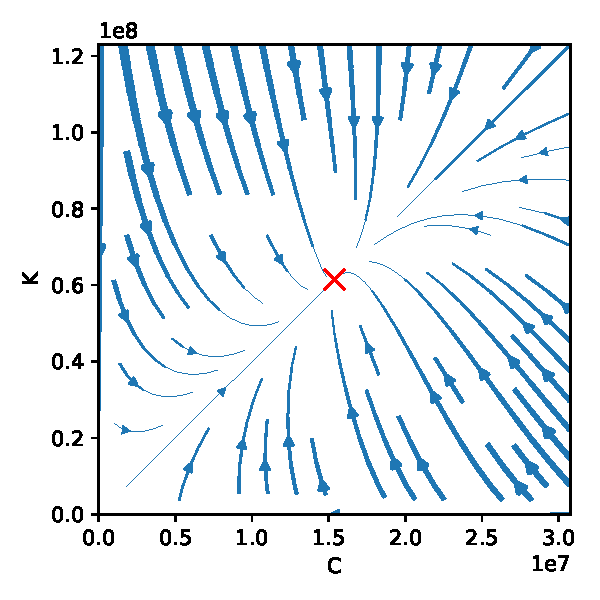
\includegraphics[width = .65 \textwidth]{./figures/phasespace.pdf}
        \caption[Phase space plot of a full clean economy]{Phase space plot of equations \eqref{eq:full_clean_ca1} and \eqref{eq:full_clean_ca2} \label{phase_space_plot}}
\end{wrapfigure}

To estimate the parameters of the model, I analyze some limiting cases of the system and compare them with real world timescales. , I can set reasonable values to some parameters.


\subsubsection{Full Clean Economy}
\label{sec:full_clean_economy}
Along the same lines, I can treat the case of a full clean economy (assuming that the fossil resource is depleted, or the households have for some other reason decided to only invest in clean capital $K_c$). \\
In this case, the equations for capital and knowledge accumulation are
\begin{subequations}
\begin{align}
    \dot{K}_c &= s b_c L^{\alpha} K_c^{\beta} C^\gamma - \delta K_c \label{eq:full_clean_ca1} \\
	\dot{C} &= b_c L^\alpha K_c^\beta C^\gamma - \chi C \label{eq:full_clean_ca2}
\end{align}
\end{subequations}
Assuming that $\alpha + \beta$ = 1, with equal elasticities for capital and labor e.g. $\alpha = \beta$, the stationary point of the system (except for the trivial one at $(0, 0)$ is 
\begin{equation}
  K_c^*= \left( \frac{\chi s}{\delta} \right) \left( \frac{s b_c^2 L}{\delta \chi} \right)^{\frac{1}{1-2\gamma}}, \qquad C^*\left( \frac{s b_c^2 L}{\delta \chi} \right)^{\frac{1}{1-2 \gamma}}
	\label{stationary_points}
\end{equation}
where the first one is non hyperbolic and the second one is stable which can be seen in the phase space plot in \cref{phase_space_plot} and the corresponding Jacobian
\begin{equation}
	J_{(K_c^*,C^*)} = 
		\begin{pmatrix}
			-\frac{1}{2}\delta & \gamma s \chi \\
			\frac{\delta}{2 s} & \chi \left(\gamma-1 \right)
		\end{pmatrix}
	\label{eq:learning_jacobian}
\end{equation}
whose Eigenvalues are strictly negative:
\begin{equation}
  \lambda_{1,2} = \frac{\delta}{2}(\gamma-1), \quad -\delta.
	\label{eq:learning_eigenvalues}
\end{equation}
The phase space plot in \cref{phase_space_plot} also suggests that there is a trajectory that satisfies 
\begin{equation}
	\frac{K_c(t)}{C(t)} = \frac{K^*_c}{C^*}
\end{equation}
meaning, one has to find a solution to the following ode:
\begin{equation}
	\dot{K}_c = s^{1-\frac{\gamma}{2}} b_c L_c^{\frac{1}{2}}K_c^{\frac{1}{2}(1-\gamma)} - \delta K_c
	\label{eq:learning_trajectory_ode}
\end{equation}
which can be done by means of separation of variables, resulting in
\begin{equation}
  K_c(t) = \left( s^{1-\frac{\gamma}{2}}\frac{b_c L^{\frac{1}{2}}}{\delta} + \exp\left[ (t_0-t) \frac{\delta (1-\gamma)}{2} \right] \right)^{\frac{2}{1-\gamma}}.
	\label{eq:learning_trajectory_solution}
\end{equation}
So, the system approaches its equilibrium approxitely exponentially from below, on a timescale that is given by
\begin{equation}
	t_c^* = \frac{2}{\delta(1-\gamma)}
	\label{eq_learning_equilibrium_timescale}.
\end{equation}
Assuming the same capital depreciation rate for clean capital as for dirty capital previously, together with $\gamma = 1/4$ which appears to be a fitting value according to \cite{Kahouli-Brahmi2008}, the timescale for clean capital accumulation is $t^*_c \approx 53 y$.

\subsubsection{Full on Dirty Economy}
\label{sec:full_dirty_economy}

Assuming, the fossil resources are very large, the dirty capital stock is significantly more profitable than the clean capital stock and subsequently all households decided to only invest in dirty capital. In this case I can treat the dirty sector isolated:
\begin{equation}
	\dot{K}_d = s I - \delta K_d, \quad I = w L + r_d K_d
	\label{eq:full_dirty_ca1}
\end{equation}
As shown before, $r_d$ is given by:
\begin{align}
	r &= \frac{\partial Y_d}{\partial K_d} - \frac{\partial c_R}{\partial K_d}, \quad c_R = b_R\left( \frac{G_0}{G} \right)^{2} R, \quad Y_d = eR, \\
	&\approx \left( 1-\frac{b_R}{e} \right)\frac{\partial Y_d}{\partial K_d},
	\label{eq:full_dirty_capital_rent}
\end{align}
and similarly for the wage $w$:
\begin{equation}
	w = \left( 1-\frac{b_R}{e} \right)\frac{\partial Y_d}{\partial L}.
	\label{eq:full_dirty_wage}
\end{equation}
So combining these, the income $I$ is equal to
\begin{equation}
	I = \left( 1-\frac{b_R}{e} \right)b_d (\alpha + \beta) L^{\alpha} K_d^{\beta}
	\label{eq_full_dirty_income}
\end{equation}
and using the assumption of zero profits e.g. $\alpha + \beta = 1$ the equation for capital accumulation \eqref{eq:full_dirty_ca1} reads
\begin{equation}
	\dot{K}_d = s\left( 1 - \frac{b_R}{e} \right) b_d L^{\alpha} K_d^{\beta} - \delta K_d
	\label{eq:full_dirty_ca2}
\end{equation}
This ordinary nonlinear differential equation can be solved by separation of variables.
\begin{equation}
  K_d (t) = K_d^{*} \left(1 - e^{(t_0-t)/t_d^{*}} \right)^{\frac{1}{\alpha}}
	\label{eq:dirty_capital_ac_solution}
\end{equation}
where the timescale for capital accumulation $t^*_d$ and the equilibrium dirty capital stock $K^*_d$ are
\begin{equation}
	t_d^{*} = \frac{1}{\alpha \delta}, \qquad K_d^{*} = \left( \frac{s b_d L^\alpha}{\delta}\left(1-\frac{b_R}{e}  \right) \right)^{\frac{1}{\alpha}}.
	\label{eq:full_dirty_capital_equilibrium_values}
\end{equation}
Since the capital depreciation rate $\delta$ is (at least for infrastructure) around 5\% p.a.\ and I assumed $\beta_d=1/2$ for the capital elasticity, the timescale for capital accumulation is $t^*_d \approx 40 y$.
%\newpage




\subsubsection{Fossil Resource Depletion}
\label{sec:resource_depletion}


For this analysis, I assume a full dirty economy like in \ref{sec:full_dirty_economy}. In addition, I assume that I can separate the timescales of resource depletion and dirty capital accumulation, e.g. I assume that dirty capital accumulation happens fast compared to fossil resource depletion such that I can approximate $K_d(t)$ with eq. \ref{eq:full_dirty_capital_equilibrium_values}. Consequently, the ode for fossil resource depletion is given by
\begin{align}
	\dot{G} &= -R \nonumber \\
        &= -\frac{b_d}{e}L^{\alpha}K_d^{*\ \beta_d} \nonumber \\
	&= - \frac{b_d}{e}L^{\alpha}\left(L^{\alpha} \frac{s}{\delta}b_d\left( 1-\frac{b_R}{e}\left( \frac{G_0}{G(t)} \right)^2 \right) \right)^{\frac{\beta_d}{1-\beta_d}}
	\label{eq:resource_deprec_approx}
\end{align}
This means that unsurprisingly, $G$ converges to a stable fix point $G^* = \sqrt{b_R/e}\ G_0$. Separating variables and substituting $g = G/G_0$ and $\varepsilon = \sqrt{b_R/e}$, the transient dynamic is given by
\begin{equation}
	\int_1^{g(t)} \frac{{\mathrm d} g'}{1 - \varepsilon^2/g'^2} = - \frac{s b_d^2 L}{e \delta G_0} \ t
	\label{eq:resource_transient_integral}
\end{equation}
To get a rough estimate of the time that it takes for the resource to deplete, I assume that $\varepsilon << 1$ and consequently for the most time, $\varepsilon^2/g'^2 << 1$.
This means that the integrand of the lhs.\ in eq.~\eqref{eq:resource_transient_integral} can be approximated by
\begin{equation}
	\int_1^{g(t)}1+\frac{\varepsilon^2}{g'^2} {\mathrm d}g' = \left[ g' - \frac{\varepsilon^2}{g'} \right]_1^{g(t)} = g(t) - \frac{\varepsilon^2}{g(t)} -1+\varepsilon^2.
	\label{eq:resource_transient_solution}
\end{equation}

\begin{wrapfigure}[23]{i}{.45 \textwidth}
    \vspace{-.8 cm}
    \hspace{-1.5cm}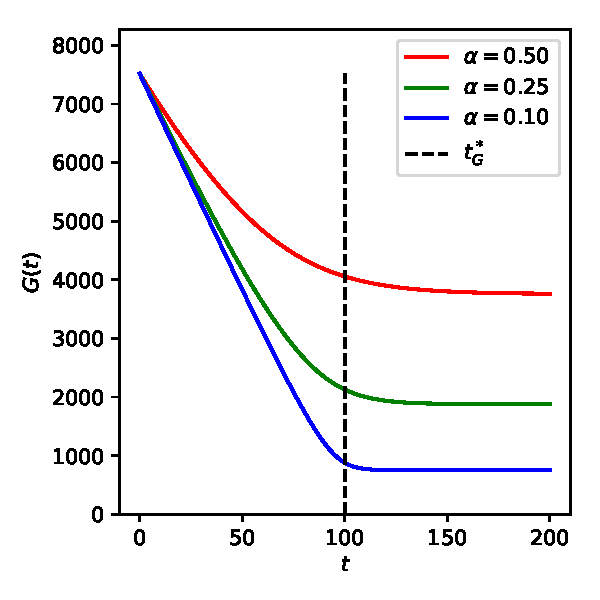
\includegraphics[width = .58 \textwidth]{figures/g_depletion.pdf}
    \caption[Resource depletion in a full dirty economy]{Resource depletion in a full dirty economy as described by eq. \eqref{eq:resource_deprec_approx}. The dashed line marks the approximate resource depletion time $t^*_G$. \label{fig:g_depletion}}
\end{wrapfigure}

This results in the implicit approximate solution:
\begin{equation}
  g(t) - \frac{\varepsilon^2}{g(t)} = 1 -\varepsilon^2 - \frac{s b_d^2 L}{e \delta G_0} \ t.
	\label{eq:resource_transient_solution2}
\end{equation}
According to this approximate solution, $g$ reaches $\alpha$ after a finite time $t^*_G$, which I use as the timescale for resource depletion:
\begin{equation}
	t^*_G = G_0\frac{e \delta}{s L b_d^2}\left( 1-\frac{b_R}{e} \right)
	\label{eq:resource_depletion_time}
\end{equation}
\Cref{fig:g_depletion} shows this resource depletion time in comparison to the numerical solution from eq. \ref{eq:resource_deprec_approx} for different values of $\alpha$ to give an impression of the goodness of the approximation.

There are different estimates for the depletion time of fossil resources ranging from approximately 60 years for crude oil to 100 years for gas and 200 years for coal.
So, I assume $t^*_G \approx 100y$. Using this, the initial resource stock $G_0$, the total population, the integrated world BIP (with an assumed growth rate of 2\%p.a.) I could get approximate estimates for $e$ and a relation of $b_d$ to  $b_R$.

% I use 2015 as the base year for my estimates. To estimate $e$ I use World GDP according to the World Bank database CITE ($75.037 \ 10^{12}$ \$) and world primary energy supply according to the BP statistical review of world energy ($13 \ 647$ Mtoe).
% Accordingly, $e$ is estimated at
% \begin{equation}
%   e \approx \frac{75.037 \; 10^{12} \; \$}{13.647 \; 10^9 \; \rm{toe}} = 5.5 \ 10^3 \left[ \frac{\$}{\rm{toe}} \right]
%   \label{ep:estimate_e}
% \end{equation}
\subsection{Parameter Values}
\label{sec:parameter_values}
\begin{sidewaystable}
	\centering
	\begin{tabular}{r|l|c|l}
          \makecell[l]{Symbol} & \makecell[l]{Default Value} & Unit & \makecell[l]{Parameter Description} \\\hline

                $\alpha_c$ & $2/3$ & & \multirow{3}{*}{\makecell[l]{Labor elasticities in the clean and dirty sector. \\Are assumed to be equal to allow for analytic \\calculation of labor shares between sectors}} \\ \hhline{---~}
                $\alpha_d$ & $2/3$ & & \\
                && & \\ \hline
                $\beta_c$ & $1-\alpha_c$ & & \multirow{2}{*}{\makecell[l]{Capital elasticities in the clean and dirty sector. Are fixed through the \\ assumption of no profits that is equivalent to $\alpha_i + \beta_i = 1$.}} \\ \hhline{---~}
                $\beta_d$ & $1-\alpha_d$ & & \\ \hline
                $\gamma$ & $1/8$ &  & Elasticity of knowledge in the clean sector.\\ \hline
                $L_1$ & $3.38 \cdot 10 ^{9}$ & billion people & Total labor in 2010. \\ \hline
                $\mu$ & 5.72 &  & \multirow{2}{*}{\makecell[l]{Exponents of resource usage $R$ and remaining \\resource stock $G$ in the resource extraction costs $c_R$. }} \\ \hhline{---~}
                 &  &  & \\ \hline
                $b_R$ & $184410.4 \cdot 10^{8}$ & \$/Mtoe & \multirow{3}{*}{\makecell[l]{Resource uptake efficiency and fossil usage efficiency for \\fossil resource. Together, they define the fraction of fossil \\resources that is not economically viable $G^* = G_0 \left(b_R/e^\rho\right)^{1/\mu}$.}} \\ \hhline{---~}
                $e$ & 4505 & \$/toe & \\
                & & & \\ \hline
                $G_0$ & $15.8 \cdot 10^5$ & Mtoe & \multirow{2}{*}{\makecell[l]{Initial and current fossil resource stock estimated from historical \\ data depicted in \cref{fig:historical_resource_use}.}}\\\hhline{---~}

                $G_1$ &  & Mtoe & \\ \hline
                $s$ & 0.25 & & Gross savings rate. \\ \hline
                $\delta $ & $5.6$ & \% p.a.  & \multirow{2}{*}{\makecell[l]{Capital depreciation rate. \\ Is assumed to be equal for both sectors}} \\
                &&\\ \hline
                $\tilde{b}_c$ &  $2.501 \cdot 10^{14}$ & U.S.\$ & \multirow{2}{*}{\makecell[l]{rescaled total factor productivity (TFP) in the clean and dirty sector. \\ as defined in eq. \ref{eq:rescalled_TFP_clean} and \ref{eq:rescalled_TFP_dirty}}} \\ \hhline{---~}
                $\tilde{b}_d$ & $5.175 \cdot 10^{14}$ & U.S. \$ & \\ \hline
                $K_{c1}$      & $2.04  \cdot 10^{15}$ & U.S. \$ & Estimated capital in the clean sector in 2010 \\ \hline
                $K_{d1}$      & $3.12  \cdot 10^{14}$ & U.S. \$ & Estimated capital in the dirty sector in 2010 \\ \hline
                $C_1$         & $7.8   \cdot 10^{14}$ & U.S. \$ & Estimated knowledge stock in the clean sector in 2010\\ \hline
                $\chi$ & 2 & \% p.a. & Knowledge depreciation rate \\ \hline
		$\tau$ & 1 & years & activity rate of households \\ \hline
		$\varphi$ & $1\leq\varphi\leq1$ & X & rewiring probability given an interaction event
	\end{tabular}
        \caption{Model parameters with description. Fitted to data from 1965 to 2010.}
	\label{tab:Heuristics_Parameter_list}
\end{sidewaystable}

To make the model results more intuitively accessible I roughly estimate the model parameters from real world data where possible. I chose 2010 as the base year, since for this year there are all the necessary estimates and data available. I do not intend to achieve any predictive accuracy with the model results and therefore use only very crude estimates for the model parameters. However, I believe that being able to express the model results at least in the right order of magnitude of real-world quantities makes also the qualitative results of the model easier to interpret.\\

First, I collect estimates for all parameters where there are values in the literature.\\

\textit{Input factor elasticities} are a defining set of parameters for Cobb-Douglas production functions. They measure the responsiveness of output with respect to a change in input factors. Historically, according to \cite{Douglas1976} the values for $\alpha$ range between approximately 0.5 and 0.75. For simplicity, I set $\alpha=2/3$ which however does not limit the generality of the approximate solutions that are developed later in section \ref{sec:Approximation} ff. \cite{Douglas1976} also states that $\alpha+\beta=1$ is a fair approximation of the actual data.
\begin{wrapfigure}[21]{i}{.55 \textwidth}
	\vspace{-.4 cm}
        \hspace{-1.5 cm}
        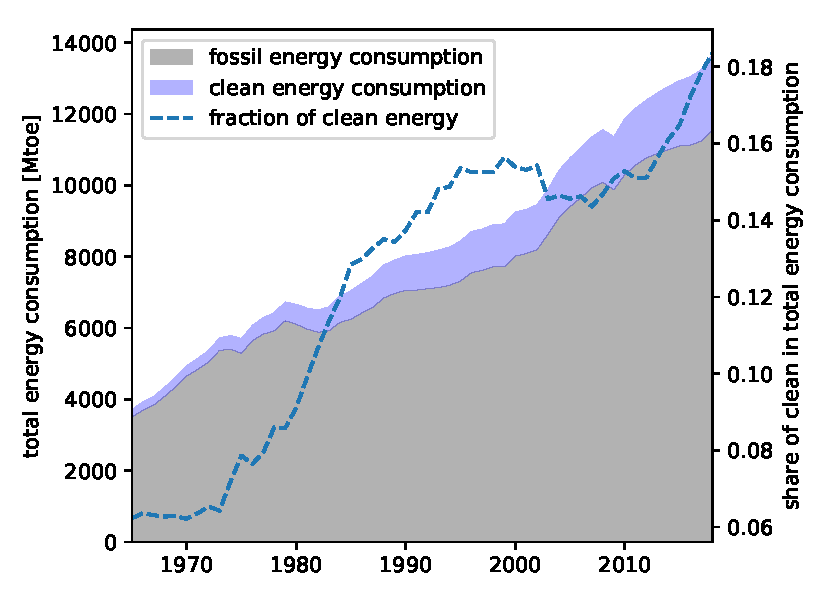
\includegraphics[width = .65 \textwidth]{./figures/energy_consumption_clean_dirty.pdf}
        \caption[Data for world energy use devided into dirty and clean sources.]{Energy usage divided into dirty (coal, oil, gas) and clean (hydro, nuclear, other renewables). The dashed line indicates the fraction of clean energy consumption. Data from \cite{dudley2019bp}.\label{fig:energy_data}}
\end{wrapfigure}
\textit{Elasticity of knowledge $\gamma$} is also the rate of learning of technology in the clean sector as discussed in \ref{sec:model_description}. This heavily depends on the technology under consideration. According to \cite{Kahouli-Brahmi2008} estimates for learning-by-doing rates approximately range between 10\% and 20\%. As an approximate value, I set $\gamma=1/8$. \\
\textit{The savings rate $s$} indicates the fraction of income that households save on average. I use a fixed savings rate for all households that is set to $s=0.25$ which is roughly in line with data for OECD countries\footnote{see \url{https://data.worldbank.org/indicator/NY.GNS.ICTR.ZS}}.\\
\textit{Total labor $L$} is taken from world bank data\footnote{see \url{https://data.worldbank.org/indicator/SL.TLF.TOTL.IN}} which estimates it at 3.38 billion people for 2016.\\
Second, I estimate parameters for which this can be done with a back-of-the-envelope calculation.\\
\textit{The knowledge depreciation rate $\chi$ in the clean sector} is assumed to be primarily a human capital effect. Therefore, I approximate the rate of knowledge depreciation with the rate workers leaving the workforce which assuming a typical career length of ~45 years results in roughly $\chi=0.02$. \\
\textit{The energy intensity in the dirty sector $e$} is estimated from world GDP\footnote{according to \url{https://data.worldbank.org/indicator/NY.GDP.MKTP.CD} world GDP was ~ $5.35 \cdot 10^{14}$ U.S. \$ for the year 2010} and the consumption of fossil ($R$) and renewable ($E$) energy\footnote{both values are taken from the BP statistical review of world energy \cite{dudley2019bp}. I count the consumption of energy from Oil, Coal and Gas as fossil and everything else as renewable.} as follows. I approximate the fraction of total economic output coming from the clean sector as the fraction of fossil energy production and estimate the energy intensity $e$ as $Y_d/R$ for the base year 2010:
\begin{equation}
  e = \frac{Y_d}{R} \approx \frac{GDP \frac{R}{R+E}}{R} = \frac{GDP}{R+E} \approx \frac{5.3 10^{14} \$}{11.9 10^9 \mathrm{toe}} = 4505 \frac{\$}{\mathrm{toe}}
  \label{eq:energy_intensity_estimate}
\end{equation}

\textit{I approximate the capital stocks in the clean and dirty sector} by assuming that the relative output of both sectors is equal to the relative consumption of fossil and renewable energy e.g. $Y_c/Y_d = E/R$. Additionally, I assume that for my purpose, national income can be sufficiently well approximated by gross production and that the capital income ratio\footnote{The capital income ration is estimated as the sum over national income by all countries divided by the estimated sum of private and national capital over all countries. For details on data and methodology, see \cite{piketty2014technical}} (CIR) of 440 \% for the year 2010 estimated by \cite{piketty2014} for the economy as a whole can be used to approximate the capital stocks of each sector individually.

\begin{equation}
  K_d \approx CIR \cdot Y_d \approx CIR \cdot GDP \cdot \frac{R}{E + R} \approx 2.04 \cdot 10^{15} ~ \textrm{U.S.} \$
  \label{eq:approx_dirty_capital}
\end{equation}

and 
\begin{equation}
  K_c \approx CIR \cdot Y_c \approx CIR \cdot GDP \cdot \frac{E}{E + R} \approx 3.12 \cdot 10^{14} ~ \textrm{U.S.} \$
  \label{eq:approx_clean_capital}
\end{equation}
\textit{The capital depreciation rate $\delta$} is assumed to be equal in both sectors. Capital depreciation rates strongly depend on the type of capital under consideration. Typical estimates range from 1.5 \% to 8.5\% for different kinds of capital see \cite{Kamps2005} and \cite{Gupta2014}. This leaves some freedom to chose $\delta$. I use this to set $\delta$ such that the estimated total capital stock $K = K_c + K_d$ together with the chosen savings rate of $s=0.25$ is an equilibrium solution to 
\begin{equation}
  \dot{K} = s \cdot Y - \delta K
  \label{eq:delta_estimate}
\end{equation} 
which results in a depreciation rate of $\delta\approx 5.68 \% \mathrm{p.a.}$.\\

\textit{I estimate the initial value of the knowledge stock in the clean sector $C$} for the base year from the time series of production in the clean sector. Production in the clean sector is approximated equivalently to eq. \ref{eq:energy_intensity_estimate} as world GDP times the fraction of clean energy consumption for the years of 1965-2010. I use the discrete version of \eqref{eq:learning_by_doing}:
\begin{equation} 
  C(t+1) = (1-\chi)C(t) + Y_c(t)
  \label{eq:discrete_clean_knowledge}
\end{equation}

to approximate the knowledge stock for the year 2010 as $C \approx 7.8 \cdot 10^{14}$ U.S. \$. \\
\begin{wrapfigure}[22]{o}{.55 \textwidth}
	%\vspace{-.4 cm}
        %\hspace{-1.5 cm}
        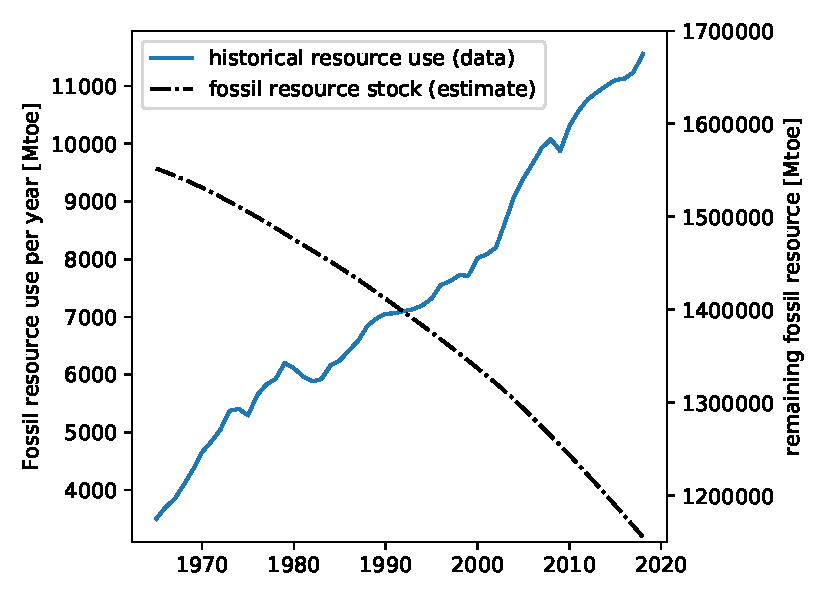
\includegraphics[width = .68 \textwidth]{./figures/fossil_resource_per_year.pdf}
        \caption[Historical data of fossil resources]{Historical data of fossil resources (coal, oil and gas) for the years 1965-2018 according to \cite{dudley2019bp} and estimated historical fossil resource stock according to eq. \ref{eq:current_fossil_resource_stock} and \ref{eq:fossil_resource_time_series}. \label{fig:historical_resource_use}}
\end{wrapfigure}
I estimate \textit{the initial fossil resource stock $G_0$ and the current resource stock $G$} for the base year from the historical usage of fossil fuels (after 1965 for which I have the data depicted in \cref{fig:historical_resource_use}) and the current estimates of fossil fuels remaining according to current use. 
There are different estimates for the depletion time of fossil resources ranging from approximately 60 years for crude oil to 100 years for gas and 200 years for coal.\\ As the model does not differentiate between different types of fossil resources, I use a depletion time of 100 years and approximate the current resource stock as the depletion time times the current fossil resource use:
\begin{align} 
  G(t=2010) 
  &\approx R(t=2010) \cdot 100, \nonumber \\
  &= 11.6 \cdot 10^{5} ~ \mathrm{Mtoe},
  \label{eq:current_fossil_resource_stock}
\end{align}
and the initial fossil resource stock as the current fossil resource stock plus the estimated cumulative resource stock according to the extrapolated fossil resource use depicted in \cref{fig:historical_resource_use}:
\begin{equation} 
  G_0 \approx G(t=2010) + \sum_{t=1965}^{2010} R(t) = 15.5 \cdot 10^{5} ~ \mathrm{Mtoe}.
  \label{eq:initial_fossil_resource_approximation}
\end{equation}

Finally, I estimate the set of remaining parameters $b_R$, $\mu$, $b_c$ and $b_d$ as follows:

I estimate the parameters of the fossil resource cost function $b_R$ and $\mu$ from historical energy price and fossil resource consumption data. I use the historical oil price\footnote{I use the yearly average oil price for different types of crude oil according to \url{https://www.statista.com/statistics/262858/change-in-opec-crude-oil-prices-since-1960/}} as proxy for the fossil resource price $p_R$ as historical data for prices for different types of fossil energy sources \citep{owidfossilfuels} shows that prices are strongly correlated and of the same order of magnitude. I create a time series of the fossil resource stock $G(t)$ from $G_0$ as estimated in eq. \ref{eq:initial_fossil_resource_approximation} and the time series of fossil resource use in \cref{fig:historical_resource_use} like

\begin{equation} 
  G(t) = G_0 - \sum_{t=1948}^{t}R(t),
  \label{eq:fossil_resource_time_series}
\end{equation}

I approximate the yearly cost of fossil resource as the product of the approximate resource price times the yearly resource use: $c_R(t) \approx p_R(t) \cdot R(t)$. 
\begin{wrapfigure}[19]{o}{.55 \textwidth}
	\vspace{-.4 cm}
        \hspace{-1.25 cm}
        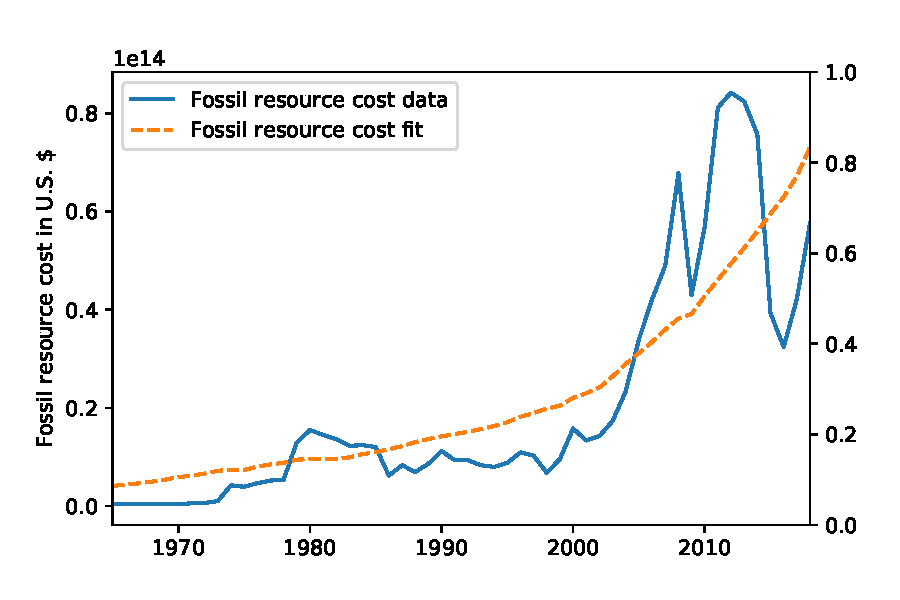
\includegraphics[width = .67 \textwidth]{./figures/resource_price_fit.pdf}
        \caption[Fit of model resource cost function to historical data]{Fit of resource cost according to eq. \ref{eq:resource_cost} to historical data generated from fossil resource use and yearly average crude oil prices as approximate fossil resource price. \label{fig:resource_cost_fit}}
\end{wrapfigure}
Then I use least squares to fit resource cost eq. \ref{eq:resource_cost} as a function of the data for resource use $R(t)$ and remaining resource $G(t)$ to the estimate data for the total resource cost $c_R(t)$ which results in 
\begin{align}
  &b_R \approx 10.4 \cdot 10^{8} \frac{\$}{\mathrm{Mtoe}} ~ \mathrm{and}\\
  & \mu \approx 5.72.
  \label{eq:estimate_resource_cost}
\end{align}
The resulting fit is given in \cref{fig:resource_cost_fit}.

To estimate the total factor productivities in the clean and dirty sector $b_c$ and $b_d$, I use equations \ref{eq:clean_production} and \ref{eq:dirty_production} and plug in the solutions for the labor shares $L_c$ and $L_d$ from equations \ref{eq:clean_labor} and \ref{eq:dirty_labor} as well as the estimates for $K_c$, $K_f$, $\alpha$, $\beta$, $\gamma$, $s$, $\delta$, $\chi$, $e$, $C$, $G0$, $G$, $b_R$, $\mu$ and the data for $R$ and $L$. Then, I can set them equal to the estimates for $Y_c$ and $Y_d$ to obtain an implicit condition for $b_c$ and $b_d$. Using numerical root finding, this results in 
 \begin{align}
  &b_c \approx 22.94 ~ \mathrm{people} ^{-\alpha} ~ \mathrm{U.S. \$}^{1-\beta-\gamma} \quad \mathrm{and} \\
  &b_d \approx 1844 ~ \mathrm{people}^{-\alpha} ~ \mathrm{U.S. \$}^{1-\beta}.
  \label{eq:estimate_total_factor_productivities}
\end{align}

Now, if you think that these units look weird, you are not alone. There is an ongoing debate between economists about sound ways to interpret total factor productivity with regards -- but not limited to -- their units. Up to the point that e.g. \cite{Barnett2007} goes so far as to state that there is no other way as to regard them in their current formulation as ``either meaningless or economically unreasonable''. Official statistics usually bypass this problem insofar as they avoid measuring levels but construct unitless growth rates for the outputs and inputs and therefore also for the residual. Inspired by this practice I will do a similar trick. I rescale the total factor productivity by dividing the input variables by typical yet arbitrarily chosen values:
\begin{align}
  Y_c &= \tilde{b}_c \left( \frac{L_c}{L_0} \right)^{\alpha} \left( \frac{K_c}{K_{c0}} \right)^{\beta} \left( \frac{C}{C_0} \right)^{\gamma} \label{eq:rescalled_TFP_clean} \\
  Y_d &= \tilde{b}_d \left( \frac{L_d}{L_0} \right)^{\alpha} \left( \frac{K_d}{K_{d0}} \right)^{\beta}. \label{eq:rescalled_TFP_dirty}
\end{align}
This brings a number of advantages. First, the rescaled total factor productivities $\tilde{b}_c$ and $\tilde{b}_d$ are measured in the same units as economic output, thereby avoiding the weird physical units from above. Second, the rescaled TFPs are independent of the input factor elasticities $\alpha$, $\beta$ and $\gamma$.
To rescale the TFPs, I will use the values of labor, capital and knowledge for the base year of the previous estimates. This results in
\begin{align} 
  &\tilde{b}_c = b_c L_0^{\alpha}K_{c0}^\beta C_0^{\gamma} = 2.501 \cdot 10^{14} ~ \mathrm{U.S. \$}, \\
  &\tilde{b}_d = b_d L_0^{\alpha}K_{d0}^\beta =              5.175 \cdot 10^{14} ~ \mathrm{U.S. \$}.
  \label{eq:rescalled_TFP_values}
\end{align}
Note, that these estimates for $\tilde{b}_c$ and $\tilde{b}_d$ can only be used in combination with the values of labor, capital and knowledge for the base year $L_0$, $K_{c}$, $K_{d0}$ and $C_0$. However, this has the advantage that these values can be changed independently from the estimates. This is very useful once I want to change the values of e.g. input factor elasticities such as the rate of learning-by-doing to evaluate their influence on the qualitative behavior of the model.\\

The parameter values that were estimated in this chapter are the foundation on which the following model analysis can be interpreted in terms of real economic quantities which hopefully helps to evaluate the findings intuitively in a sociopolitical and economic context of the twenty first century.
Still, both the model and the parameter estimates are obviously oversimplified for exact quantitative predictions but quantitative predictions were never the goal of the model.

\iffalse
\subsubsection{Opinion spreading in the adaptive voter model}
A common way to describe the dynamics of the adaptive voter model in terms of macroscopic variables is the pair approximation.
For simplicity, lets assume a system with two possible opinions $A$ and $B$, on a network with $N$ nodes and $K$ edges.
I describe the model using a vector $(x, y, z)^T$:
\begin{equation}
	x = \frac{[A]-[B]}{N}, \quad y = \frac{[AA]-[BB]}{K}, \quad z = \frac{[AB]}{K}
	\label{avm_variables}
\end{equation}
There are four possible events in the system
\begin{itemize}
	\item 1. an A node rewiring,
	\item 2. a B node rewiring,
	\item 3. an A node adapting a B node and 
	\item 4. a B node adapting an A node.
\end{itemize}
The probabilities for these events to happen are
\begin{align}
	p_1 &= \varphi\frac{z(1+x)}{2(1+y)}, \quad p_2 = \varphi \frac{z (1-x)}{2(1-y)} \\
	p_3 &= (1-\varphi)\frac{z(1+x)}{2(1+y)}1/2({\mathrm tanh}(\Delta I)-1),\\
	p_4 &= (1-\varphi)\frac{z(1-x)}{2(1-y)}1/2({\mathrm tanh}(-\Delta I)-1)
	\label{avm_event_ps}
\end{align}
and their influence on the state vector $s = (x, y, z)^T$ are $s' = s + s_i$ with $s_i$ one of the following:
\begin{align}
	s_1 &= \colvec{3}{0}{1}{-1}, \quad s_3 = \colvec{3}{-2}{-2k\frac{1+y}{1+x}}{-1+2k\frac{1-y-2z}{1-x}-\frac{1-y-2z}{1-y}}\\ 
	s_2 &= \colvec{3}{0}{-1}{-1}, \quad s_4 = \colvec{3}{2}{2k\frac{1+y}{1+x}}{-1+2k\frac{1-y-2z}{1-x}+\frac{1-y-2z}{1-y}}
	\label{avm_event_effects}
\end{align}
Such that in the limit for large N, one gets deterministic equations for $x$, $y$ and $z$:
\begin{align}
	\frac{\dot{x}}{\tau} =& -(1-\varphi)\frac{z}{2}\frac{1-x}{1-y}(\mathrm{ tanh}(\Delta I)-1) + (1-\varphi)\frac{z}{2}\frac{1+x}{1+y}(\mathrm{ tanh}(-\Delta I)-1) \\
\frac{\dot{y}}{\tau} =& \quad \varphi\frac{z}{2}\left( \frac{1+x}{1+y} + \frac{1-x}{1-y} \right) + (1-\varphi)kz\left( \mathrm{ tanh}(-\Delta I) - \mathrm{ tanh}(\Delta I) \right) \\
	\frac{\dot{z}}{\tau} =& -\varphi\frac{z}{2}\left( \frac{1+x}{1+y} + \frac{1-x}{1-y} \right) \nonumber \\
	& + (1-\varphi)\frac{z}{2} \left[ \frac{1+x}{1+y} \frac{1}{2}(\mathrm{ tanh}(\Delta I)-1) \left( (1+y-2z)\left( \frac{2k}{1+x}-\frac{1}{1+y} \right)-1 \right) \right. \nonumber \\
	& \hspace{1.9 cm} + \left.\frac{1-x}{1-y}\frac{1}{2}(\mathrm{ tanh}(-\Delta I)-1)\left( (1-y-2z)\left( \frac{2k}{1-x}-\frac{1}{1-y} \right)-1 \right)  \right]
	\label{avm_ode}
\end{align}
assuming that the income difference $\Delta I$ between different cue orders is sufficiently large, this can be reduced to
\begin{align}
	\frac{\dot{x}}{\tau} =& -(1-\varphi)\frac{z}{2}\frac{1-x}{1-y} \\
\frac{\dot{y}}{\tau} =& \quad \varphi\frac{z}{2}\left( \frac{1+x}{1+y} + \frac{1-x}{1-y} \right) + (1-\varphi)kz \\
	\frac{\dot{z}}{\tau} =& -\varphi\frac{z}{2}\left( \frac{1+x}{1+y} + \frac{1-x}{1-y} \right) \nonumber \\
	& + (1-\varphi)\frac{z}{2} \left[ \frac{1+x}{1+y} \left( (1+y-2z)\left( \frac{2k}{1+x}-\frac{1}{1+y} \right)-1 \right) \right]
	\label{avm_ode_reduced}
\end{align}
and from this one can see that the timescale for $x$ to reach its equilibrium values is roughly 
\begin{equation}
	t_a^* = \tau(1-\varphi)
	\label{avm_timescale}
\end{equation}
Since, at least according to my impression, people don't really change their minds or make new friends too often, I propose keeping this timescale between $1<t_a^*<10$ years.
\fi
\newpage
\subsection{Opinion formation and decision making}
\label{sec:oppinion_formation_and_decision_making}

I assume that households use the Take-the-Best heuristic as explained in section~\ref{sec:intro_bounded_rationality} to decide whether to invest their savings in the clean or the dirty sector. This assumption results in three follow up questions that have to be answered for the model setup. A) Which cues i.e. bits of information to the households use to compare the two sectors for their decision? B) Which combinations of these cues (i.e. which cue orders) do I want to model? C) Which initial distribution of cue orders should I use as an initial condition. This chapter will answer these three questions in this order.

To represent the cue order in the model and in this text, I assign numbers to the different cues $(c_l)$ and represent cue orders $O$ as lists of these numbers: $O: (c_l,\dots c_m)$. As a rule, cues only appear once in each cue order and if one cue definitively discriminates between options, there will be no other cues after it.

\subsubsection*{A) Which information do households use to compare the clean and the dirty sector for their investment decision?}
I assume that households use information that is available to them either in their own mind such as inherent norms and preferences as well as information that is available to them in their surroundings such as factual data about their economic performance of the clean and the dirty sector or the behaviour of their acquaintances.\\

\textit{Inherent norms:}
I assume that it is an option for households to invest in one or the other sector purely out of their inherent conviction to do so, disregarding all other information that might be available. This constitutes two cues: 
\begin{itemize}
  \item [ $(0)$ ] the household invests its savings in the clean sector, regardless of all other information,
  \item [ $(1)$ ] the household invests its savings in the dirty sector, regardless of all other information.
\end{itemize}
Both of these cues definitively discriminate between the two sectors.\\

\textit{Factual data about the economic performance of the clean and the dirty sector:}
Many behavioral investment models such as \cite{Lux1999}, \cite{Alfarano2008a}, \cite{Chiarella2011a} and \cite{Hommes2017BoomsPrices} assume two possible ways to make investment decisions and hence model two types of investors - for an overview see e.g. \cite{Hommes2006a} or \cite{Chakraborti2011}. Such models usually assume that investors either invest based on their beliefs about an inherent value of an investment (such investors are called fundamentalists as they believe in an inherent fundamental value of an asset and that the asset price will return to this value eventually) or based on their beliefs on a future value of an investment (such investors are called chartists as they do believe that asset prices are inherently volatile and that their future price can best be read out out of the price time series - the chart).
Motivated by this approach, I assume that households can use either the current value of an investment to ground their decision or they can use an estimate about which of the investments will be more valuable in the future. I also assume that they use the current return rates $r_c$ and $r_d$ as a proxy for the inherent value of an investment in the clean or the dirty sector and that they use their first derivatives with respect to time $\dot{r}_c$ and $\dot{r}_d$ as a proxy for the future development of the value of an investment in one or the other sector. I implement these as the two following cues:
\begin{itemize}
  \item [$(2)$] households invest in the sector whose capital return rate is distinctly higher e.g. $r_j > (1+\iota) r_k$,
  \item [$(3)$] households invest in the sector whose trend in capital return rates is distinctly more positive e.g. $\dot{r}_k > (1+\iota) r_k$,
\end{itemize}
and with distinctly, I mean $\iota = 0.1$.\\

\textit{Behavior of households' acquaintances:}
As discussed previously in section \ref{sec:investment_decision_making}, I assume that one of the households different drivers is homophily, i.e. the desire to be similar to ones acquaintances. I have already used this in the motivation of the social learning component where households are homophilic with regards to their beliefs that are represented by their cue orders. To be consistent, I use it again here where I say that one possible driver for households investment decision is that they want to behave similar to their acquaintances. This behavior is also referred to as `Imitate the Majority' in the heuristic decision making literature see e.g. \cite{Gigerenzer2009} \cite{garcia2009does} and \cite{Gigerenzer2011}. 
I implement this in terms of the following cue:
\begin{itemize}
  \item [$(4)$] A household invests its savings in the sector in which the majority of its acquaintances invest e.g. it invests in the sector $k$ if $\sigma_k > 0.5 + \iota$
\end{itemize}
with $\sigma_k$ being the fraction of acquaintances investing in sector $k$ and again $\iota=0.1$.

\subsubsection*{B) Which cue orders to consider in the model?}
With regards to the cue orders in the model, there is a trade off to consider. For a high number of cue orders, one needs a considerably higher number of households to get enough households to use each cue order to get meaningful results in terms of statistics. But a higher number of households leads to significantly more costly numerical simulations. (For a short study of model run times in its current implementation depending on the number of simulated households, see \cref{fig:runtime}.) Therefore, I will not consider all possible cue orders\footnote{All possible combinations would be $5!=120$, however since cues 0 and 1 end the heuristic, only $38$ of these cue orders are distinct.}, but I will restrict the model to cue orders of length two\footnote{I hypothicise that only a vanishing fraction of decisions would be made with more than two cues and that making these decisions at random (as the TTP Heuristic prescribes it) instead of with more cues does not make a difference. I could track the fraction of decisions that are made at random for an ensemble of simulations at some point to prove this.}. Additionally, of all $14$ remaining possible cue orders of length $2$, I only consider a subset. This subset must still represents all possible cues and should therefore be sufficient to answer the question of how different possible grounds for an investments
\begin{wrapfigure}[23]{o}{.4 \textwidth}
	\vspace{-.4 cm}
        \hspace{-1.9 cm}
        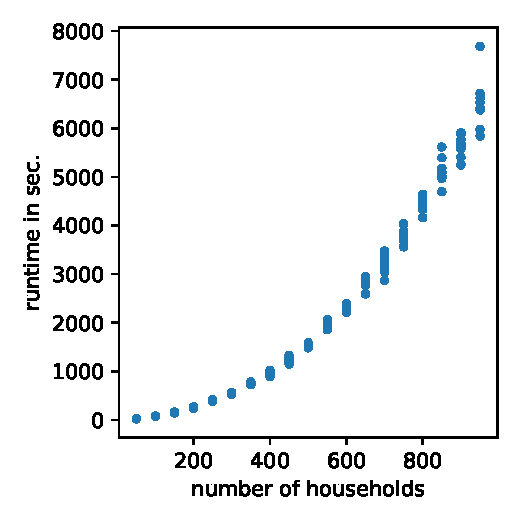
\includegraphics[width = .55 \textwidth]{./figures/runtime.pdf}
        \caption[Model run time depending on number of households]{Run times of the model in my implementation (Python) depending on the number of households modelled.\label{fig:runtime}}
\end{wrapfigure}
decision that are prevalent in the population influence the aggregate behavior of the social-economic system with regards to a possible rapid decarbonization transition.\\

Overall, I consider three different types of households. First, households that ground their decisions based on financial incentives e.g. that consider cues $(2)$ and $(3)$ in different order. Second, I consider households that ground their investment decision on homophily, but fall back to other discriminating information, if there is no clear majority amongst their acquaintances e.g. they use cue $(4)$ first and one of the other cues second. Finally, I consider households that invest in one or the other sector out of an inherent preference, e.g. they use cue $(0)$ or $(1)$ and no other cues, since these cues are always decisive. \\

To sum up, I consider the following set of eight cue orders and for a more intuitive description also the following names for the households using them:
\begin{itemize}
  \item [$(2, 3)$]: myopic investor,
	\item [$(3, 2)$]: trend sensitive investor,
	\item [$(4, 2)$]: myopic herder,
	\item [$(4, 3)$]: trend sensitive herder,
	\item [$(4, 1)$]: Green conformer,
	\item [$(4, 0)$]: Conservative conformer,
	\item [$(1)$]: `Gutmensch',
	\item [$(0)$]: Redneck
\end{itemize}
With this set of cue orders, the remaining question is their frequency among the population of households.

\subsubsection*{C) Which initial distribution of cue orders should be used?}

The initial condition for the heterogeneous households consists of the distribution of cue orders, the distribution of the different kinds of capital and the configuration of the acquaintance network. This determines the investment decisions of the individual households and consequently the fraction of savings that is invested in the two economic sectors. \\
Arguably, to yield realistic results, the initial fraction of savings that goes into the two economic sectors should be consistent with the economic situation and historical data that the parameters of the economic model were fitted to. On the one hand, considering this situation, there is no actual data on the relative shares of investment. However, since I chose the parameters such that the total capital stock is in equilibrium subject to investment and depreciation according to eq. \ref{eq:delta_estimate}, it is sufficiently close to require that the relative shares of the capital stocks in the two sectors $K_c(t)/K_d(t)$ remains approximately constant.\\

\begin{figure}[t]
  \centering
  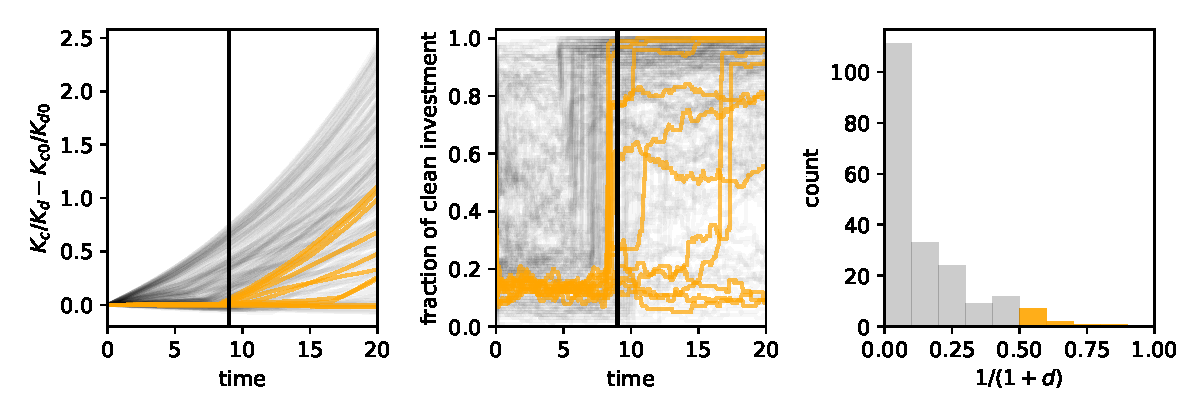
\includegraphics[width= \textwidth]{figures/initial_condition_sampling.pdf}
  \caption[Trajectories of N=200 runs with initial conditions for cue orders sampled from an uninformed prior]{\textbf{Trajectories of N=200 runs with initial distribution of cue orders sampled from an uninformed prior.} Panel a shows the distance of the simulated relative shares of capital $K_c(t)/K_d(t)$ from the initial condition. Panel b shows the fraction of total investment going into the capital stock of the clean sector. Panel c shows the distribution of closeness as defined by eq. \ref{eq:distance_criterion} and eq. \ref{eq:closeness} for the simulated trajectories.}
  \label{fig:initial_conditions_sampled}
\end{figure}
Therefore, I want to find an initial distribution of cue orders that likely leads to an aggregate ration of clean and dirty investment that keeps the ration of capital in the two sectors constant.\\

To find an initial distribution of cue orders that is likely to fulfill this criterion of an approximately constant ratio of capital in the two sectors, I use a method that is loosely inspired by Bayesian updating. Put simply, I first sample the initial distribution of cue orders from an uniformed prior then second, simulate the resulting model trajectory and calculate its distance $d$ to the formalized criterion and third, I calculate the weighted sum over the sample of initial cue order distributions using the inverse of the distance as weight to use it as the actual initial condition.



More precisely, I define the initial distribution of the 8 different cue orders by their relative frequencies $Q: [n_1, \cdots n_8]$ among the households. Given a fixed number of households $H$, the set of possible cue order distributions is equal to the discrete points on the 7 dimensional hyperplane that is given through $H = \sum_i n_i, n_i \in \mathbf{N^{+}}$. To get an equally distributed sample of these points $Q_m$, I use a Dirichlet distribution $\mathrm{Dir}(\mathbf{\alpha})$ with $\mathbf{\alpha}=(\alpha_1, \cdots \alpha_8), ~ \alpha_i=1$. I then randomly assign a cue order to each households according to their frequencies as given by $Q_m$. I also randomly assign equal shares of either clean or dirty capital each household - independent from their assigned cue order. Finally, I use an Erd\H{o}s-Renyi random graph with $p=0.1$ as the initial acquaintance network between households where acquaintance relations are set independent of the households' cue orders.


\begin{table}[t]
    \centering
    \begin{tabular}{c|c|l}
        Relative frequency & Cue order & Name \\ \hline
        $0.145$&$(2, 3)~$&myopic investor\\
    $0.075$& $(3, 2)~$& trend sensitive investor\\
        $0.124$& $(4, 2)~$& myopic herder\\
        $0.118$& $(4, 3)~$& trend sensitive herder\\
        $0.139$& $(4, 1)~$& Green conformer\\
        $0.166$& $(4, 0)~$& Conservative conformer\\
        $0.074$& $(1)~$& `Gutmensch'\\
        $0.158$& $(0)~$& Redneck

    \end{tabular}
    \caption{Fitted initial cue order distribution in terms of relative frequencies.}
    \label{tab:initial_cue_order_dist}
\end{table}

For these initial conditions, I simulate model trajectories for the years 2010-2030. For these trajectories, I calculate the distance to the chosen criterion of constant relative capital stocks between the sectors as as the Euclidean distance for the years 2010-2019:
\begin{equation}
  d_m = \sqrt{\sum_{t=2010}^{2019}\left( \frac{K_c(2010)}{K_d(2010)} - \frac{K_{c,m}(t)}{K_{d,m}(t)} \right)^{2}}.
  \label{eq:distance_criterion}
\end{equation}
I chose the years 2010-2019, as I would argue that looking back at the last decade, a major decarbonization transition is yet to come.
\Cref{fig:initial_conditions_sampled} a) shows the relative shares of capital for a sample of $M=200$ initial cue order distributions $Q_m$ with the one that can be considered close to the desired criterion highlighted in orange. In quantitative therms, I define closeness $cl$ as
\begin{equation}
  cl = \frac{1}{1+d}
  \label{eq:closeness}
\end{equation}
and consider a trajectory to be close if $cl > 0.5$.
The resulting initial distribution of cue orders $Q_r$ that hopefully fulfills the desired criterion is then calculated as
\begin{equation}
    Q_r = \frac{1}{\sum_m \frac{1}{d_m}}\sum_{m}\frac{1}{d_m} Q_m.
  \label{eq:updated_cue_order_distribution}
\end{equation}
The resulting cue order distribution is given in table \ref{tab:initial_cue_order_dist}.
Note that this only sets the relative frequencies of cue orders and does not determine the microscopic configuration of acquaintance relations, initial capital distribution and individual cue order assignment.

\begin{figure}[t]
  \centering
  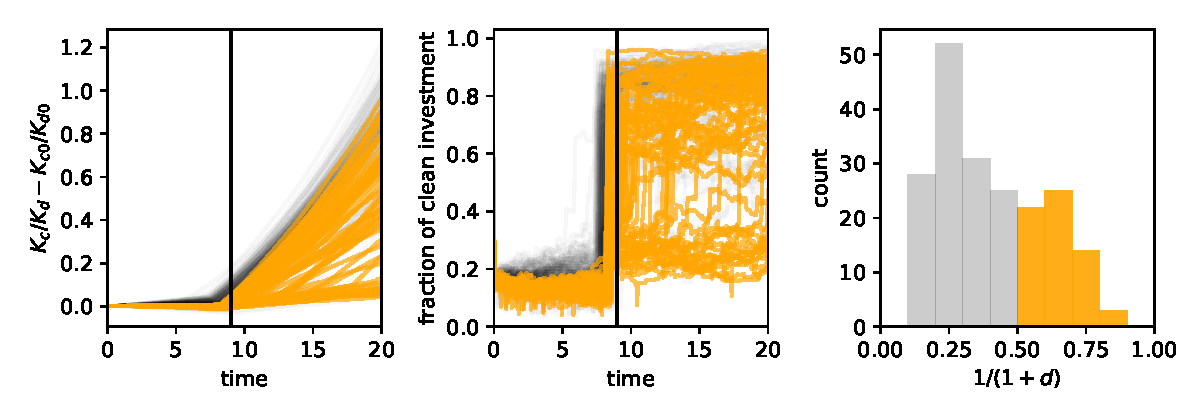
\includegraphics[width= \textwidth]{figures/initial_condition_fitted.pdf}
  \caption[Trajectories of N=200 runs with updated initial conditions]{\textbf{Trajectories of N=200 runs with updated initial conditions.} Initial relative frequencies of cue orders are calculated as to the weighted sum of the initial relative frequencies in \cref{fig:initial_conditions_sampled}. The weighs are the inverse distances as defined by eq. \ref{eq:distance_criterion}.}
  \label{fig:initial_conditions_fitted}
\end{figure}

To determine the success of this procedure, I simulate an ensemble of trajectories with the resulting $Q_r$ and display the trajectories in \cref{fig:initial_conditions_fitted} analogously to the results from uniformly distributed $Q_m$ in \cref{fig:initial_conditions_sampled}. Again, I highlight the trajectories that I consider `close' to the desired criterion. Comparing the distributions of closeness $cl$ in \cref{fig:initial_conditions_sampled} c and \cref{fig:initial_conditions_fitted} c, some things are apparent. First, sampling initial $Q_m$ from an uniformed prior results in a Poisson like distribution of closeness $cl$ for the resulting trajectories with the majority of trajectories exhibiting far from constant relative shares of capital in the two sectors and Second, the `posterior' $Q_r$ results in dramatic improvements in terms of closeness meaning that I can consider approximately one third of the trajectories as `close' e.g. $cl>0.5$ and only a vanishing fraction as `far' e.g. $cl<0.1$.\\

%A third fact that comes as a surprise to me is found in fig \ref{fig:initial_conditions_fitted} b. Here, it becomes apparent that most of the simulated trajectories exhibit a major opinion swing around 9 years into the simulation from households investing primarily in the dirty sector to households investing primarily in the clean sector. To me, this timing coincides so stunningly well with the Fridays-for-Future movement -- even more so, as I would call the model conceptional and the parameter fitting crude that I feel I have to emphasise that I did not put this behavior into the model in the first place.

\section{Results}  
In the previous section, I have fitted parameters of the model to reproduce realistic conditions in terms of resource extraction, capital stocks in the clean and dirty sector and economic production for the year 2010. I have also fitted initial conditions that are likely to reproduce the status quo until around the year 2019 insofar, as they keep the relative shares of capital in the clean and dirty sector approximately constant. 

In the following section, I will have a closer look at the actual model dynamics and possible qualitative insights from the structure of the transformation process that it depicts.

\subsubsection{The Default Scenario}
\label{sec:default_scenario}
\Cref{fig:default_alpha_05} shows results from an ensemble of 1000 runs with 100 households for the parameters and initial conditions that I have outlined in the previous two sections. These results -- especially the fraction of total investment that goes into the clean sector -- 
\begin{wrapfigure}[26]{o}{.5 \textwidth}
	\vspace{-.1 cm}
        \hspace{-1.8 cm}
        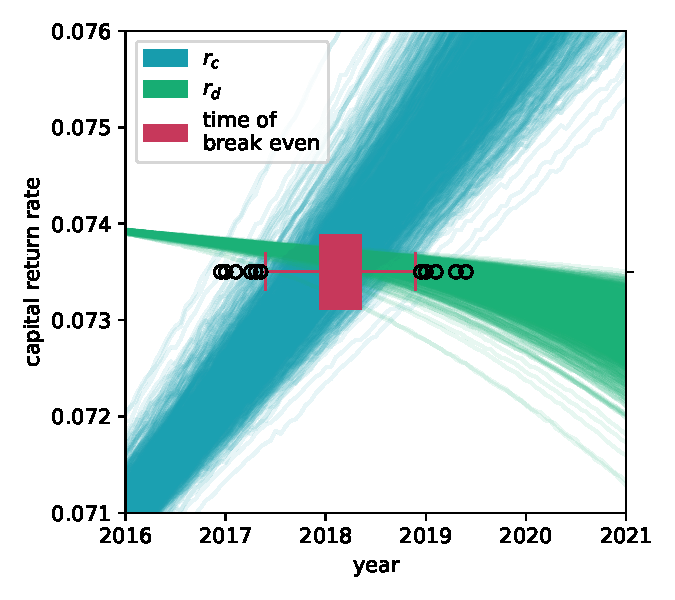
\includegraphics[width = .64 \textwidth]{./figures/break_even.pdf}
        \caption[Capital return rates in the clean and dirty sector for N=1000 runs]{Capital return rates in the clean and dirty sector for M=1000 runs. Statistical properties of the distribution of intersection times between the return rates in the two sectors are indicated with a box plot.\label{fig:break_even}}
\end{wrapfigure}
%results show social tipping behavior
show a rapid switch in many trajectories from investment primarily in the dirty sector before 2018 to investment primarily in the clean sector after 2018. 

% this social tipping behavior most likely works as follows
This rapid switch is most likely caused by the following mechanism. As shown in \cref{fig:break_even}, the return rate of capital $r_c$ in the clean sector exceeds the return rate of capital $r_d$ in the clean sector in or around the year 2019 -- primarily due to increasing productivity of capital as a result of learning by doing in the sector that increases the knowledge stock $C$. Consequently, households that are `myopic investors' and therefore invest in the sector with the higher capital return rate start to invest their savings in the clean sector. If these households are sufficiently connected to other households that are `herders' or `conformers', the latter may follow their example. Therefore, even though the fraction of myopic investors may be small (their initial frequency is only 1/8th), the fact that their example may be followed by those that decide according to the behavior of their surroundings (whose combined initial frequency is about 1/2) can lead to rapid tipping in the investment behavior of 

the majority of households. This also explains the heterogeneity in final outcomes. As the rapid switch in investment depends on the decision making of households that rely on imitation of the majority of their neighbors, this tipping process is heavily influenced by the micro structure of the model -- particularly the structure of the acquaintance relations between households.

\begin{figure}[H]
	\centering
        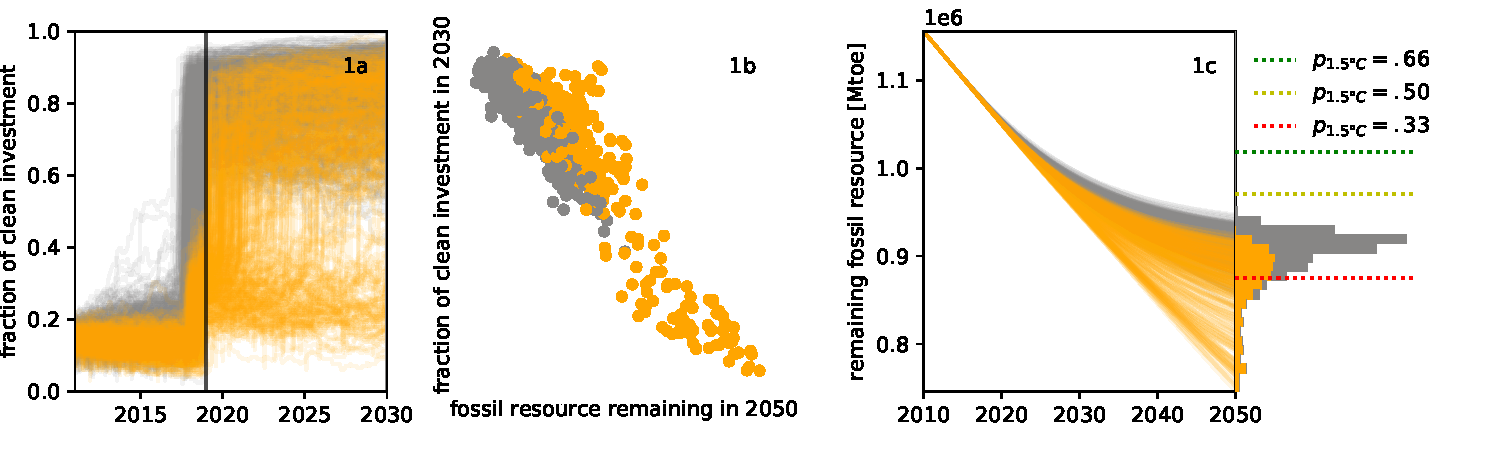
\includegraphics[width = 1.2 \textwidth]{figures/fitted_initials_evaluation05.pdf}
        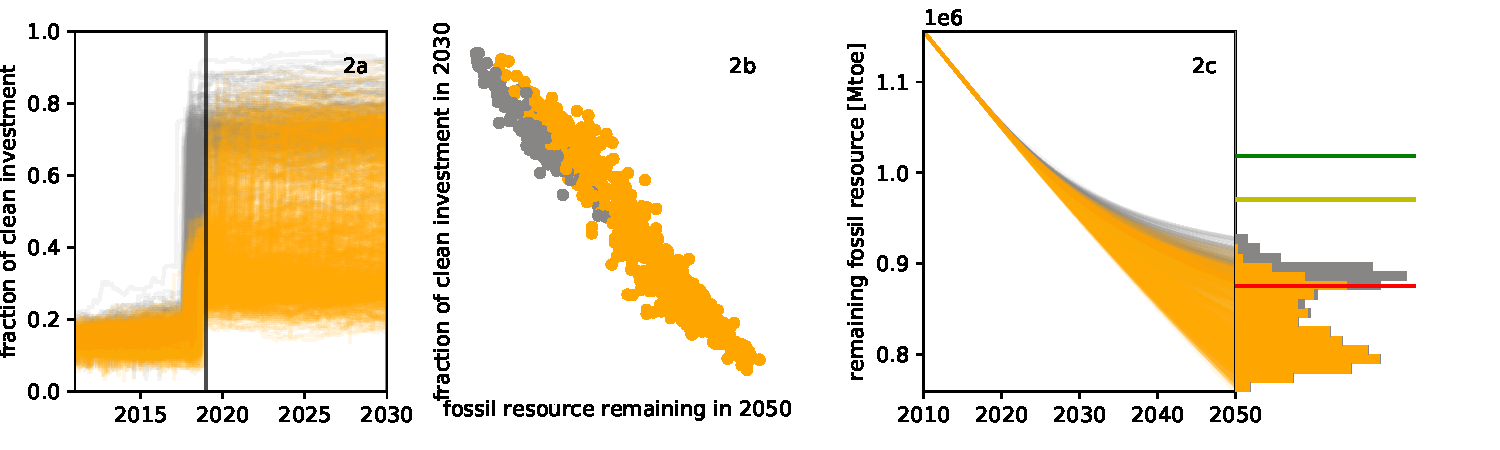
\includegraphics[width = 1.2 \textwidth]{figures/fitted_initials_evaluation07.pdf}
        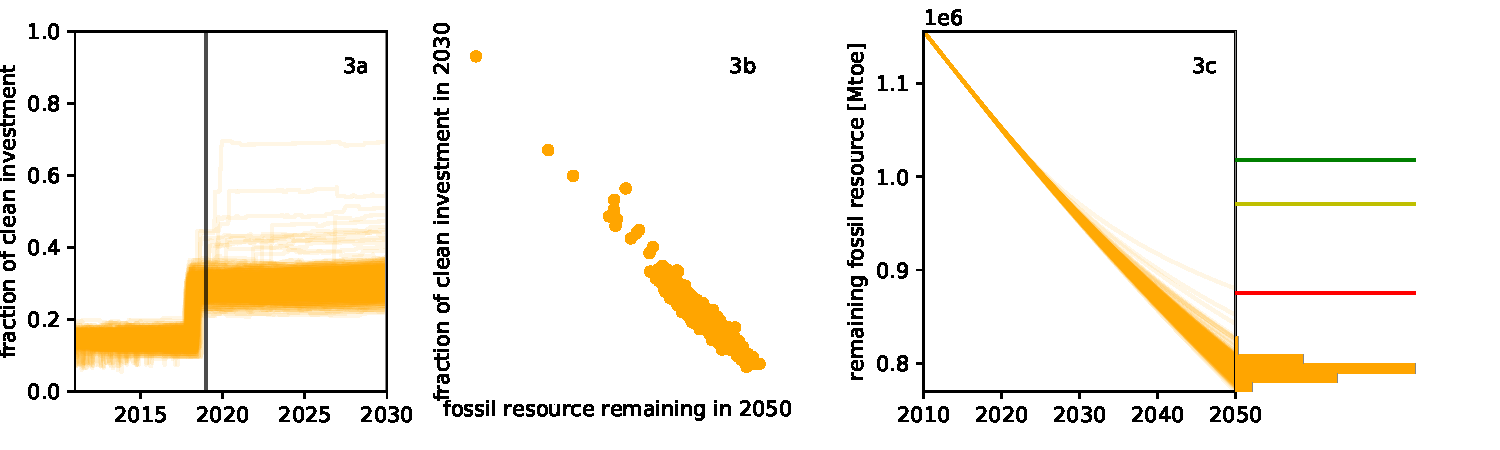
\includegraphics[width = 1.2 \textwidth]{figures/fitted_initials_evaluation09.pdf}
        \caption[Trajectory of decarbonization transition depending on the network rewiring rate in the social learning process]{\textbf{Decarbonization transition depending on rewiring probability $\gamma$}. Panels 1, 2 and 3 each show ensembles of M=1000 runs with N=100 households, for different rewiring probability 1: $\varphi=0.5$, 2: $\varphi=0.7$ and 3: $\varphi=0.9$. Other parameter values and initial conditions as described in section \ref{sec:parameter_values} and \ref{sec:oppinion_formation_and_decision_making}. Results from runs where the fraction of clean investment exceeds 50\% before 2019 are colored grey. All other results are colored orange. The x and y distributions on the scatter plot in panels b are equal to the distributions of trajectories on the right y axis in panels a and c respectively. The stacked histogram attached to panels c gives the relative frequencies of the bundle of trajectories i.e. the distribution of remaining fossil resource in 2050 over the ensemble of simulations. The dotted lines in these histograms indicate the emission budgets for the $1.5\circ$C target according to IPCC 2013}
        \label{fig:default_alpha_05}
\end{figure}



% tipping in investment only slowly leads to reduction in emissions
Panel 1c shows that this switch of the direction of investment is then later followed by a reduction of the use of the fossil resource. The time lag between the switch of investment and the reduction of resource use is due to the fact that the existing physical capital $K_c$ in the dirty sector is still in productive use and only gradually depreciating over a timescale of approximately $t_{d}^{*}\approx 50$ years as I have shown in section \ref{sec:full_dirty_economy}. It is also clear that not all simulation runs follow this switching behavior and that in a number of runs the majority of investment continues to go to the dirty sector over the entire simulation period or only switches to the clean sector substantially later.

% to set cumulative resource use in perspective, I compare them to emission targets
To set these results into perspective, I have converted the emissions budgets from the IPCC2013 report \citep{stocker2013climate} for the $1.5^{\circ}C$ target roughly into their equivalents in tonnes of oil equivalent in fossil resource use. I show three budgets that are estimated to keep global warming under $1.5^{\circ}$C with different probabilities $p$ and indicated them as dotted lines with the distribution of cumulative resource use on the right edge of panel c. For the conversion, I have used a value of 0.43 metric tonnes CO2 per barrel of crude oil\footnote{https://www.epa.gov/energy/greenhouse-gases-equivalencies-calculator-calculations-and-references} and the definition of one barrel as 0.136 tonnes according to OPEC standards\footnote{https://www.opec.org/library/Annual\%20Statistical\%20Bulletin/interactive/current/FileZ/cfpage.htm}.
In the following, I will call the different budgets
\begin{itemize}
  \item T1 for $p=0.66$ to stay below $1.5^{\circ}$C warming,
  \item T2 for $p=0.5$ to stay below $1.5^{\circ}$C warming and
  \item T3 for $p=0.33$ to stay below $1.5^{\circ}$C warming.
\end{itemize}


% this shows that in the model under the (very optimistic) business as usual scenario, results are bad.
Comparing the results of the model runs in row 1 of \cref{fig:default_alpha_05} with the emission budgets it is apparent that this business as usual scenario of the model exceeds the T2 budget at any rate and even exceeds the T3 budget in many cases. Note that this business as usual scenario can be considered rather optimistic as it assumes technological progress only in clean technologies, and also note that many runs that stay within the T3 budget are colored gray which means that in these cases social tipping happened before 2019. This I would argue is not what happened in the real world and can therefore be considered unrealistic. More to the contrary, if the trigger for a major change in investment from dirty to clean technology will be their relative returns, this would mean that tipping might happen even later in the real world, because e.g. \cite{Farmer2016} predict that this point will only be somewhere between 2025-2030.

% and they get even worse, if the clustering of likeminded households increases.
For the model runs in the first row of \cref{fig:default_alpha_05} it was equally likely for households to break a link and to establish one with a like-minded individual as it was to communicate and possibly update their beliefs if they encountered a differently minded household. 
However, different studies on real world social network data indicate that individuals tend to form clusters of like-minded individuals \citep{girvan2002community, Lerman2010, Law2011, Takhteyev2012}.

Rows 2 and 3 show the dynamics of the model in case the probability for like-minded households to form clusters increases, e.g. for increasing rewiring probability $\varphi$. These results support the previous discussion of the social tipping dynamics depending on the connection between households that rely on economic indicators for their decisions and households that rely on the observation of their peers. If the rewiring probability increases, households that conform with their neighbors cluster together and tend to form groups that self-stabilize in their behavior.

Also, households that use economic indicators to inform their decisions do the same and therefore cannot communicate their decision (in terms of observable behavior) and experience (in therms of generated income) to others. As a result, for $\varphi=0.7$ this leads to a scenario where in some simulations the information can still propagate through the acquaintance network and lead to a social tipping event whereas in other simulations this does not happen, leading in sustained investment in the dirty sector. As a result, the final distribution of cumulative resource use in 2050 is bimodal and runs that exhibit tipping have a chance to stay within the T3 budget while those that do not exhibit tipping exceed it.

If the rewiring probability further increases to $\varphi=0.9$, at the time when investment in the clean sector becomes more profitable, only a fraction of households switch investment to the clean sector. This indicates that propagation of this behavior through the network fails because the network is already too fragmented into unconnected components which is also in line with the segmentation transition that has been shown by \cite{Rogers2013, Wiedermann2015, Klamser2016} and \cite{Min2017} for adaptive voter type models.\\

\textbf{To sum up:}
\begin{itemize}
  \item Decisions of a number of informed individuals in combination with others that rely on the observation of their peers can lead to social tipping in the model given that the tendency of like-minded individuals to cluster together is sufficiently low.
  \item Regardless, in the (rather optimistic) default scenario of the model, emissions are likely to exceed the budget that would keep global warming below $1.5^{\circ}$C with a probability of $p=0.5$.
  \item Especially a tendency of like-minded individuals to cluster together leads to a certain failure to stay within the budget that would keep global warming below $1.5^{\circ}$C with a probability of $p=0.33$ given the model assumptions.
  \item To conclude, in the model world, technological progress and individual choice of households are very unlikely to prevent global warming above $1.5^{\circ}$C.
\end{itemize}



\begin{figure}[t]
    \centering
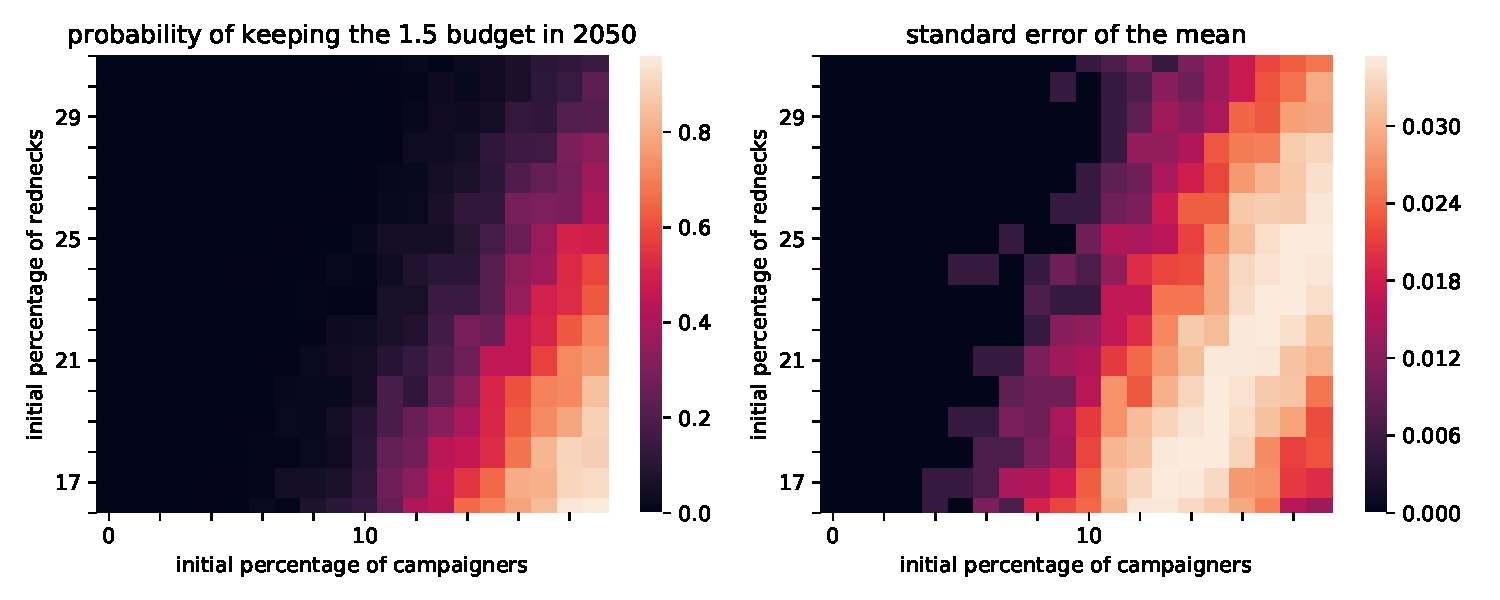
\includegraphics[width = \textwidth]{figures/p_budget15p50_in2050.pdf}
\caption[Probability of staying within the p=0.5, 1,5 degree budget in 2050 depending on the initial size of a campaign in 2010]{Probability of staying within the p=-1.5, 1.5 degree budget in 2050 depending on initial size of campaign in 2010 and initial fraction of rednecks.}
    \label{fig:p15in2050}
\end{figure}

\subsubsection{A Campaign for Clean Investment}
\label{sec:campaign}
The previous section has shown that given the models' assumptions it is unlikely that cumulative fossil resource usage will stay below what is necessary to prevent global warming above $1.5^{\circ}$C. In a default scenario with technological progress in clean technology and individual investment decision making most simulated trajectories exceeded the emissions budget T3 associated with a $p=0.33$ chance of keeping global warming below $1.5^{\circ}$C even for a moderate tendency of like-minded households to cluster together. For higher tendencies of clustering, the modeled economy almost surely exceeds this budget as soon as 2050 without a tendency to slow down fossil resource use.\\

This section will discuss if in the model a social movement in favor of clean investment can drive social tipping to clean investment sufficiently to stay within at least the T2 budget associated with a $p=.5$ chance to keep global warming below $1.5^{\circ}$C.\\

Currently, campaigning against the use of fossil fuels takes different forms: \\

Movements like \textit{Extinction Rebellion} and \textit{Ende Gel\"{a}nde} use non-violent means of civil disobedience to stop the economic operation of fossil fuel companies -- especially in the lignite business -- to draw public and media attention to the matter and to influence the public discourse in favor of legislations that limit or prohibit the use of fossil fuels.\\

\textit{Fridays for Future} originated as a student school strike and grew into a coordinated movement that protests to pressure politicians to enact legislations that are in line with the proposals by the IPCC to mitigate global warming.\\

The \textit{Fossil Fuel Divestment Movement} uses classical campaigning tools to advocates the withdrawal of financial capital from firms that are associated with the extraction and burning of fossil fuels. This campaign -- however well intended -- suffers from difficulties. First, even if financial capital is divested from those firms, the physical capital is still there and in operation and potential buyers may be even less inclined to vote for corporate social responsibility. Also previous studies by \cite{Ans2013} suggest that the intended pressuring effects on stock prices that would keep fossil fuel firms from raising new capital necessary for further resource exploration might be small. \cite{SIF2014Report} estimates that only approximately 15 \% of investors invest subject to socially responsible guidelines and that divested holdings are, especially in liquid markets, very likely to quickly find their way to less responsible investors.\\

These campaigns have in common that they want to influence public opinion in favor of mitigating climate change and that they build on a strong mindset of sustainable individual behavior.\\

\begin{wrapfigure}[25]{i}{.45 \textwidth}
	\vspace{-.4 cm}
        \hspace{-1.4 cm}
        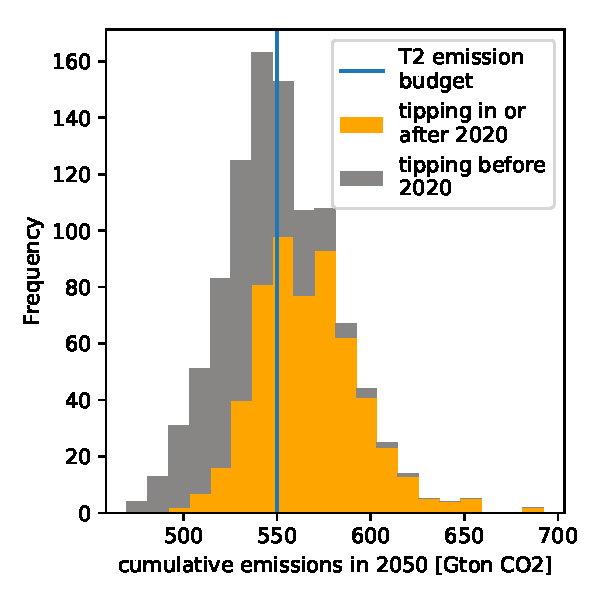
\includegraphics[width = .57 \textwidth]{./figures/emissions_with_campaign.pdf}
        \caption{Stacked histogram for distribution of final cumulative emissions in 2050 for initial campaign sizes between 10\% and 15\% compared to T2 emissions target. \label{fig:campaign_sucess}}
\end{wrapfigure}

To better understand the possible effects of such campaigning efforts, I implement a social movement/campaign in the model. I measure the success of the campaign as the probability to keep emissions within the T2 budget and analyze the dependence of 
this probability on factors such as the fraction of opposing opinions among the other households, accompanying political measures and the probability of like-minded households to form homogeneous clusters.\\

I implement the campaign in the model in the following way: Members of the campaign will act sustainably e.g. they always invest in the clean sector out of inherent preference (just like the households acting as 'Gutmensch'). In addition, they will not imitate any other reasoning for their behavior. Besides that, members of the campaign interact with other households in the way that is prescribed by the adaptive voter dynamics.\\
\Cref{fig:p15in2050} shows the likelihood of staying within the T2 emissions budget in 2050 depending on the initial size of the campaign in 2010 vs. the initial fraction of opposing opinions ('rednecks'). This shows that for the fraction of opposing opinions of $~15\%$ that I have estimate in section \ref{sec:oppinion_formation_and_decision_making}, emissions can only stay within the T2 budget if the initial campaign size comprise more than $~10\%$ of the population and almost certainly stay within the T2 budget only if the initial size of the campaign exceeds $~15\%$ of the population. Additionally, if the initial fraction of opposing opinions increases linearly, the initial size of the campaign has to increase linearly as well to have the same effect on cumulative emissions.\\

However, a closer look at the results for campaign sizes $n_cp$ between $10\%$ and $15\%$ shows that for many trajectories that stay within the T2 emissions budget tipping happens in or before 2019. To illustrate this, \cref{fig:campaign_sucess} shows the final cumulative emissions in 2050 $E_{2050}$ averaged over $n_{cp}$ between $10\%$ and $15\%$ compared to the T2 emissions budget. The results for trajectories where tipping happens in or before 2019 are given in grey as opposed to the results for trajectories where tipping happens after 2019 that are given in orange. Tipping is classified as the point in time $t_{c90}$ where more than $90\%$ of investment goes into the clean sector e.g. the point in time where investment in the dirty sector is essentially stopped. This shows that in the model the probability to stay within the T2 emissions budget averaged over these campaign sizes of $p(E_{2050}<\mathrm{T2}|10\% \leq n_{cp} \leq 15\%) \approx 0.5$ reduces to $p(E_{2050}<\mathrm{T2}|10\% \leq n_{cp} \leq 15\%, t_{c90}>2019) \approx 0.3$ if one only considers model results where tipping didn't happen before 2019 as I would argue that this is unrealistic.

\begin{figure}[t]
    \centering
    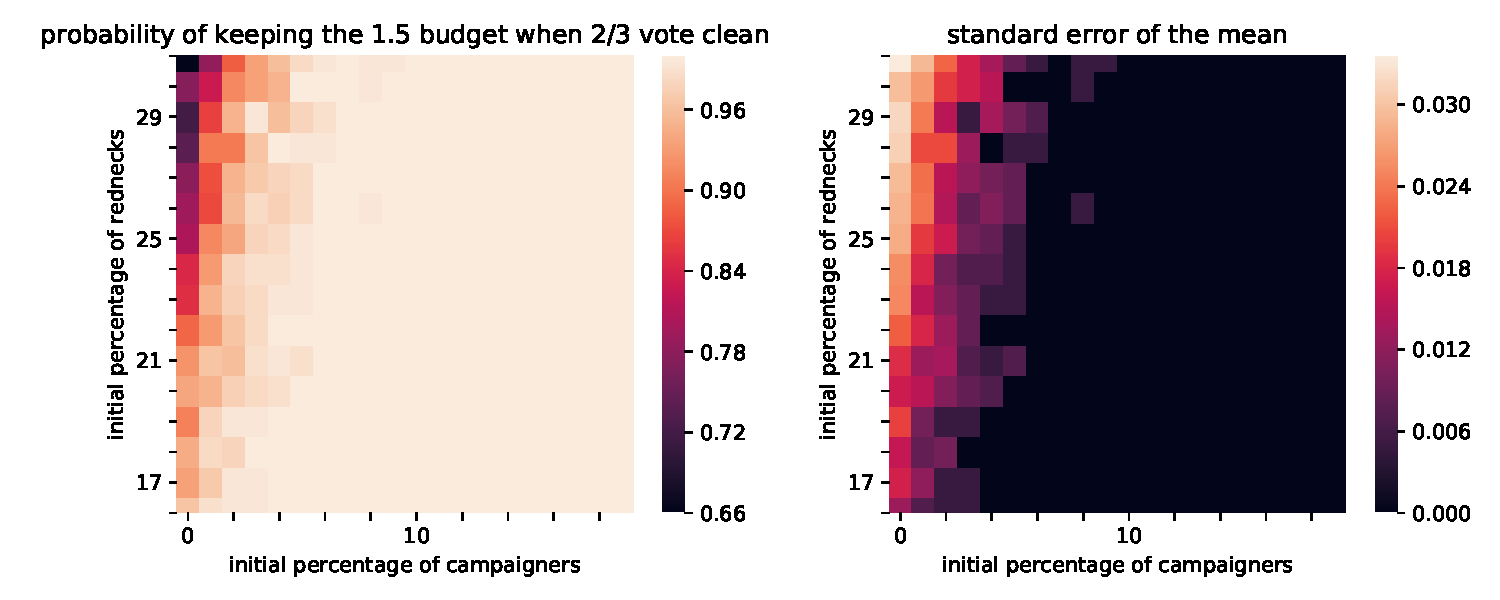
\includegraphics[width = \textwidth]{figures/p_budget15p66_at_campaign_success.pdf}
    \caption{Probability of staying within the p=0.5, 1.5 degree budget when 2/3 of households vote clean depending on the initial size of campaign in 2010 and initial fraction of rednecks.}
    \label{fig:p15sucess}
\end{figure}

The discussion of results presented in \cref{fig:p15in2050,fig:campaign_sucess} indicates that in the model campaigning efforts that aim at norm changes to alter public opinion and individual behavior alone have little prospect of success. However all of the campaigning efforts that I have mentioned above also aim at change in public policy. Therefore, I estimate the likelihood of the success of campaigning efforts that also result in a change in public policy under the most ideal circumstances. Ideal circumstances meaning that as soon as $2/3$rd of the population invest in the clean sector a public policy is implemented that prohibits the further exploration of the fossil resource. This is very optimistic as it neglects vested interests of individuals due to their existing capital in the dirty sector that would be rendered idle by this policy, resulting in a reduction of income of individuals of up to $30\%$.


\Cref{fig:p15sucess} shows the likelihood of cumulative emissions to stay within the T2 budget at the point in time when $2/3$rd of the population decide to stop investing in the dirty sector depending on the initial size of the campaign and the initial fraction of opposing opinions in the population. This shows that as soon as the initial size of the campaign is non-zero, shutting down technologies that rely on fossil fuels as soon as a qualified majority of the population stops investing in them, this would almost surely keep cumulative emissions within the T2 budget. These results show also that even a substantial amount of opposing opinions does not critically endanger the success of the campaigning efforts as even for an initial fraction of $~30\%$ of the population investing in the dirty sector out of their inherent conviction, an initial size of $~1\%$ of the population that takes part in the campaign is sufficient to almost surely lead to social tipping in favor of the clean sector before the T2 budget is exceeded.

This shows that in the model campaigning in combination with strict public policy at the soonest point in time when it would possibly be politically viable is in principle capable of preventing global warming above $1.5^{\circ}$C.
However, political realities show that public policy is rarely as strict as banning an entire sector at once and that it usually comes with substantial interim periods to reduce potential fallout to a minimum. Also, bans are usually the ultima ratio and policy makers usually prefer methods that rely on voluntary self-commitment and technological change as long as possible.

\begin{figure}[t]
    \centering
    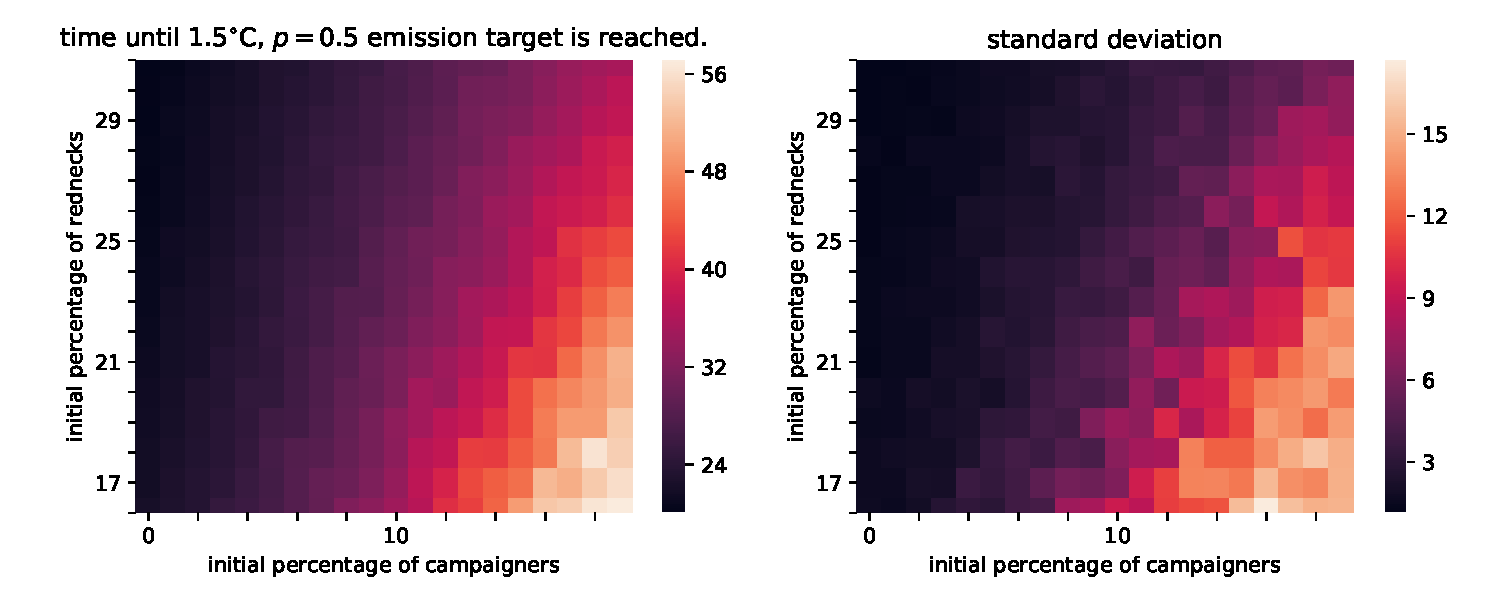
\includegraphics[width = \textwidth]{figures/time_until_emissions_target.pdf}
    \caption{Time until the p=0.5, 1.5 degree budget is used up depending on the initial size of campaign in 2010 and initial fraction of rednecks.}
    \label{fig:time_until_budget_reached}
\end{figure}

Therefore, I want to analyze how long campaigning efforts could possibly elongate the window of opportunity for softer policy measures before dirty technologies would eventually have to be banned to stay within the T2 budget. \Cref{fig:time_until_budget_reached} shows the time until the T2 budget is reached depending on the initial size of the campaign and the initial fraction of opposing opinions in the population. 
\begin{wrapfigure}[26]{o}{.45 \textwidth}
	\vspace{-.4 cm}
        \hspace{-1.4 cm}
        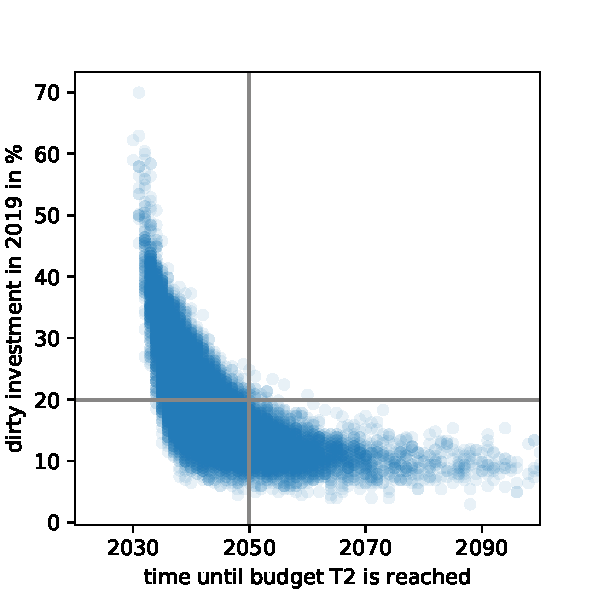
\includegraphics[width = .57 \textwidth]{./figures/dirty_investment_consequences.pdf}
        \caption{Scatter plot of percentage of investment in the dirty sector vs. the time until the T2 emissions budget is reached for an initial fraction of opposing opinions of 16\% to $20\%$ and an initial fraction of campaigners of $10\%$ to $15\%$. \label{fig:dirty_investment_consequences}}
\end{wrapfigure}
These results show that for an initial fraction of opposing opinions of $~15\%$ as projected in section \ref{sec:oppinion_formation_and_decision_making}, campaigning can increase the time window substantially from until 2023 with no initial campaign in 2010 to up to until 2066 if the initial campaign size in 2010 were $~15\%$ of the population. 
However, the elongation of the time window for clean technologies to establish on a voluntary basis would come from essentially halting almost all investment in dirty technology as soon as 2019 to only use the existing capital stock in the dirty sector until it depreciates. \Cref{fig:dirty_investment_consequences} shows the fraction of dirty investment in 2019 vs. the time until the T2 emissions budget is reached. 
Here, it is apparent that less then $20\%$ of investment in the dirty sector in 2019 is a necessary, yet not sufficient condition for the extension of the time frame until the T2 budget is exceeded beyond 2050. In simple words this means that every car that is sold today reduces the probability that this same car (or any other brand new car for that matter) could be used until the end of its life cycle should one seriously intend to keep emissions within the T2 budget.

Finally, I want to examine how the tendency of like-minded households to form clusters influences the probability of success of a campaign that advocates clean investment. Therefore, \cref{fig:campaign_phi} shows the mean and standard deviation of cumulative emissions at the success of the campaign e.g. when 2/3rd of households invest in the clean sector for varying initial size of the campaign and the rewiring probability $\varphi$. Here, a rewiring probability of $\varphi<0.6$ e.g. a low to medium tendency of like-minded households to cluster together has little to now effect on the prospects of campaigning efforts. However, if the rewiring probability increases, the model exhibits a transition to a state where campaigning efforts become futile for a campaign that starts with less than $15\%$ of participation in 2010. This is not surprising, as e.g. \cite{Rogers2013, Wiedermann2015} and \cite{Klamser2016} have shown before that for a rewiring probability $\varphi$ above a critical value, adaptive voter type network dynamics undergo a segmentation transition where an initially fully connected graph decomposes into smaller unconnected sub graphs of nodes that share the same state/opinion. This also happens in this model -- somewhat attenuated by the exploration behavior of households that acts as noise to the adaptive voter dynamics and therefore facilitates some connection between otherwise disconnected homogeneous clusters of households.\\

In this light, the fact that an initial campaign size of $20\%$ can still lead to social tipping e.g. 2/3rd of households investing in the clean sector can be explained by the models initial conditions. Initially, the acquaintance graph between households is fully connected and household opinions are set regardless of the network topology. This fully connected network needs some time to decompose into disconnected clusters which in return means that there is a limited time frame in which social tipping can happen. This however also means that this effect is somewhat artificial since -- given the assumption of homphilic association among households holds -- real networks would exhibit some correlation of clustering and individual traits already in their initial conditions.\\

\begin{figure}[t]
    \centering
    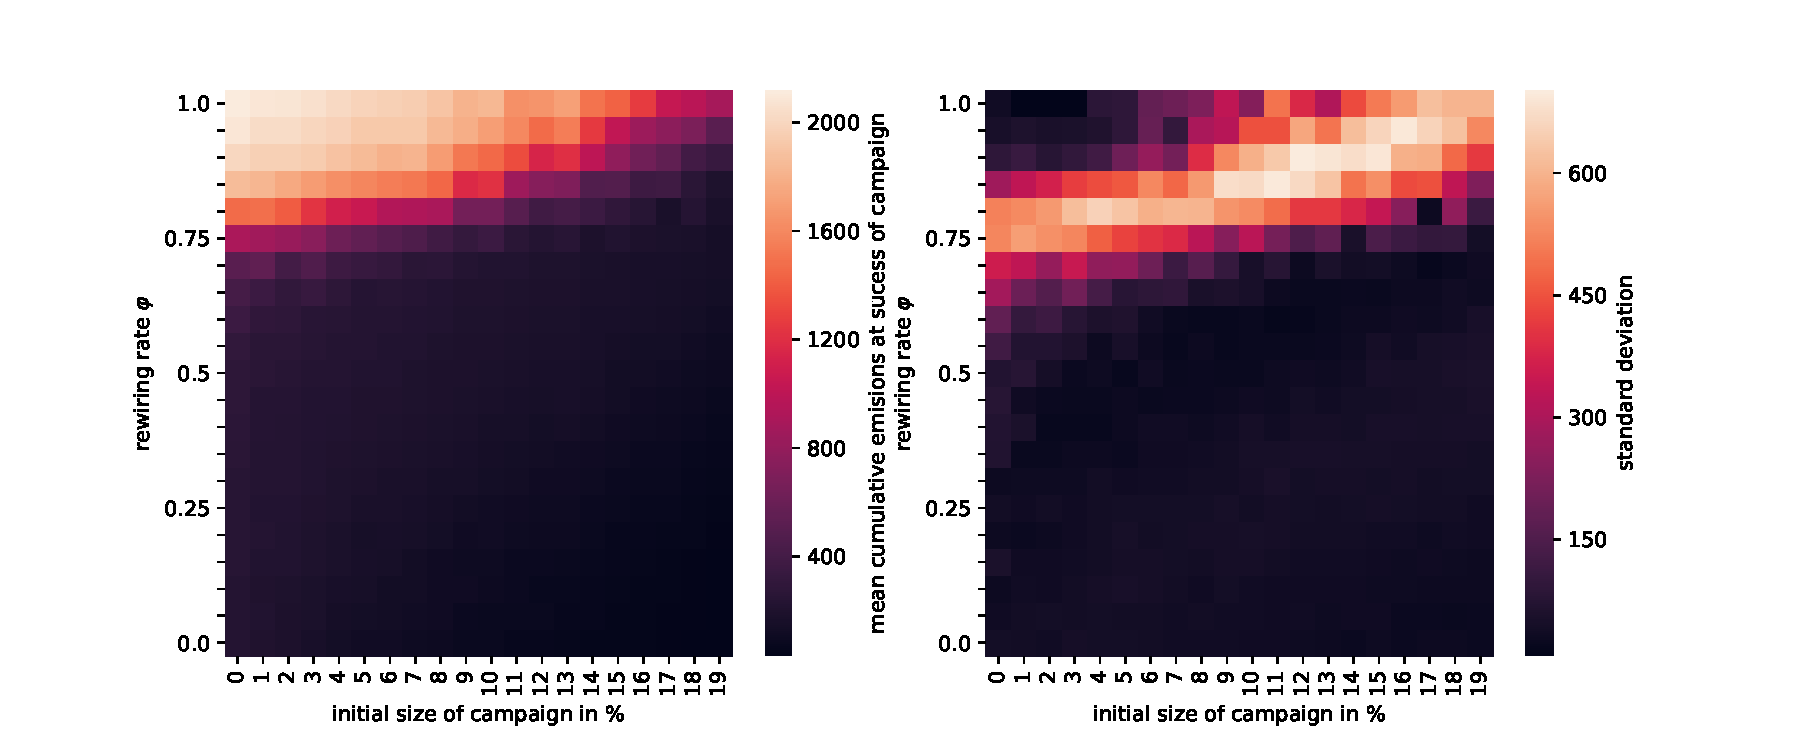
\includegraphics[width = \textwidth]{figures/campaign_vs_phi.pdf}
    \caption{Mean and standard deviation of cumulative emissions at the success of the campaign depending on the initial size of the campaign and the rewiring probability $\varphi$ that is a parameter for the tendency of like-minded households to cluster together. }
    \label{fig:campaign_phi}
\end{figure}

To sum up, I showed that in this model:
\begin{itemize}
  \item Campaigning to stop investment in dirty technologies alone has little to no chance to prevent global warming above $1.5^{\circ}$C if climate change mitigation only happens through technological progress and individual decision making.
  \item Complementing a campaign, a strict public policy that prevents the use of fossil resources has the potential to limit global warming below $1.5^{\circ}$C if it is implemented as soon as it is politically opportune e.g. as soon as a qualified majority of 2/3rd of households invest in the clean sector.
  \item Even though campaigning cannot prevent global warming above $1.5^{\circ}$C, it can substantially extend the window of opportunity to come up with less strict measures to halt the use of fossil fuels given that it successfully halts investment in the dirty sector.
  \item In the model, the dependence of the prospects of success of campaigning efforts on the dendency of like-minded individuals to cluster together is highly nonlinear due to a segmentation transition in the underlying adaptive voter dynamic.
\end{itemize}

\section{Discussion and Conclusion}
\label{sec:heuristics_conclusion}

% what did i do (maybe also shortly reiterate why)
In the previous chapter, I developed, calibrated and analyzed a model that combines social learning and individual, bounded rational decision making with elements of neoclassical economics to model sustainability transitions away from fossil fuels.
In the model, heterogeneous households are owners of capital and labor that they use to generate income. The households save a fixed amount of their income and decide between a `clean' and a `dirty' sector in which they can invest their savings. The `dirty' sectors uses a fossil resource for production whereas the `clean' sector uses a clean technology that is still under development. In this stylized production economy, capital rents and wages in the two sectors as well as fossil resource use in the dirty sector form subject to aggregated supply and demand of labor and capital.
In this context, the model describes the interplay of social dynamics and individual processing of information from different sources that lead to collective behavior of individuals. This collective behavior in return shapes the environment in which the modelled individual live.
In contrast to many other social-ecological models, this model differentiates between judgement and action of individuals. In most social-ecological models that emulate individual opinion formation, behavior, opinion and action are equivalent and spread via imitation of successful behavior. In contrast, in this model individuals learn heuristics that they use to judge which action would be best given the circumstances.

% how did i do it
I used adaptive network dynamics for social learning, ordinary differential equations with algebraic constraints to model economic dynamics economic dynamics and fast and frugal heuristics to describe individual decision making individual decision making.
I solved the algebraic constraints of the model analytically and I roughly estimated parameters from data where possible. I complemented this with the analysis of different limiting scenarios to estimate the parameter dependence of timescales for different processes in the model and I conducted numeric experiments to analyze the models default behavior.
I implemented a social movement in the model in which members of the movement only ever invested in the clean sector and did -- unlike the other households -- not change their judgement heuristic subject to the social learning process. Subsequently, I conducted different numeric simulation experiments to analyze the prospects of success of such a campaign in the given model subject to different parameters and potential accompanying public policy measures.

% what are shortcomings of the model
The model that is developed and analyzed in this chapter is conceptual and as such it is stylized and oversimplified in many respects.
For instance it does not consider any climate damages and does not differentiate between different fossil resources and sources of emissions. Its economic model is simplistic as in reality many kinds of physical capital are not explicitly connected to a specific sector and can be reallocated. Also, investment decisions are rarely as simple as deciding between two sectors to invest in. Rather, making investment decisions has increasingly become a science of its own.\\
Considering these shortcomings of the model, its results should by no means be understood as actual predictions. However, it still pictures general trends and allows insights into effects that emerge from interactions of different processes that are -- at least in this combination -- usually not considered together.

% what were the results
The results of the numeric simulations that I conducted indicate that given the underlying assumptions of the model, campaigning efforts that advocate investment in carbon free technologies alone have only a very limited chance of mitigating global warming above $1.5^{\circ}$C as in realistic scenarios they are unable to limit cumulative emissions to the T2 budget that limits global warming below $1.5^{\circ}$C with a probability of $p=0.5$ in the IPCCs projections.
Measuring the cumulative emissions at the point in time when two thirds of households started to invest in the clean sector however suggest that if at this point a public policy could be implemented to ban the use of fossil fuels, cumulative emissions could be kept within the T2 budget almost certainly. 
Unsurprisingly, the evaluation of these experiments also shows that campaigning that leads to reduced investment in fossil fuel dependent technology in favor of increased investment in clean technologies increases the window of opportunity that could be used for mitigation measures that are softer than a ban before the T2 budged is exceeded.

% what is the significance of the results in a broader context
The results give hope that it might be possible to still mitigate global warming above $1.5^{\circ}$C and strongly suggest that to this end a number of different, complementary measures will be needed. They suggest that a timely phase out of investment in technologies that rely on fossil fuels is a crucial step to mitigate global warming. The suggest that for public opinion to swing in favor of clean technologies, these technologies have to be viable and competitive also in the short term. This can and already has been facilitated with appropriate subsidies, market design and taxation. The results also suggest that at some point certain dirty technologies will have to be shut down and that capital associated with these technologies will have to be written of. This is already happening -- in Germany at least -- but might have to happen sooner and on a much larger scale to actually have the desired effects on cumulative emissions. Finally, the results strongly suggest that campaigning can help to influence individual decisions and public opinion to an extent that makes the aforementioned measures politically viable and their consequences less severe. But the results also indicate that strong clustering of like-minded individuals such as in political polarization and the formation of filter bubbles that allow completely disconnected and fragmented discourses to coexist can render such campaigning efforts entirely futile.

% what else can be done.
In the analysis of the model, I considered a combination of campaigning and public policy measures that are aimed to ban the use of fossil fuels. However, a model along these lines would also allow to analyse the effects of a number of other policy measures.
Obvious candidates would be taxation for dirty and subsidies for clean technologies similar to \cite{Geier2019}. A not so extensively yet interesting policy measure would be marketing strategies such as nudging and priming that aim to influence an individuals internal evaluation of different options and often time explicitly anticipate heuristic decision making. Priming for instance aims to activate certain concepts in individuals' minds to make them consider aspects related to this concept over other unrelated aspects in their decisions. In this framework such measures can be implemented by temporarily altering individuals' cue orders after exposure to marketing efforts.

% what can be done better
To make this model more realistic, one could consider a number of improvements and extensions. With regards to the economic dynamics, one can consider technological progress also in the dirty sector as well as a possible third sector that does not depend on either of the two technologies. For instance production of energy could be divided into fossil and renewable energy production and production of final goods can happen in a separated sector as e.g. in \cite{Heitzig2015a}. In individual decision making natural extensions would be the consideration of more possible cues and the full spectrum of the resulting cue orders as well as other modi of decision making such as alternative heuristics that fit the decision environment (such as tallying) or to consider more sophisticated decision strategies (such as utility maximization in combination with Bayesian updating) to take account of the fact that especially bigger investors certainly use more complex and elaborated decision making tools. With respect to social learning one can consider the fact that in this model individual parameters are homogeneous between agents. However in real world systems the preference for homphilic rewiring is likely to be heterogeneous between individuals. For instance empirical studies on Optimal Distinctiveness Theory \cite{hornsey1999subgroup, leonardelli2010optimal} find that the preference for relationships with individuals with similar traits is heterogeneous within the groups under study.
Also, one can consider that individuals may not only learn how do decide where to invest but maybe also how much. With that regard, the subsequent chapter will elaborate on the interesting possible effects of individuals that use social learning to set their savings rate in a one sector production economy.
